\section{Validation with $\xi_{\pm}$}
\label{sec:validation}



This section presents a comparison between theoretical predictions and measurements in the simulations for all our 6 models. We include here the statistical error obtained from covariance matrix computed analytically as described in \citet{KiDS1000_Joachimi}, which includes contributions from the Gaussian, non-Gaussian and super-sample covariance terms, assuming survey properties that match our simulation in terms of area, shape noise, galaxy density, tomographic $n(z)$ and cosmology.   The diagonal elements are used to assign the error bars in our figures, and the full matrix is used in the MCMC analyses presented in Sec. \ref{sec:inference}.

%---------------
\begin{figure*}
%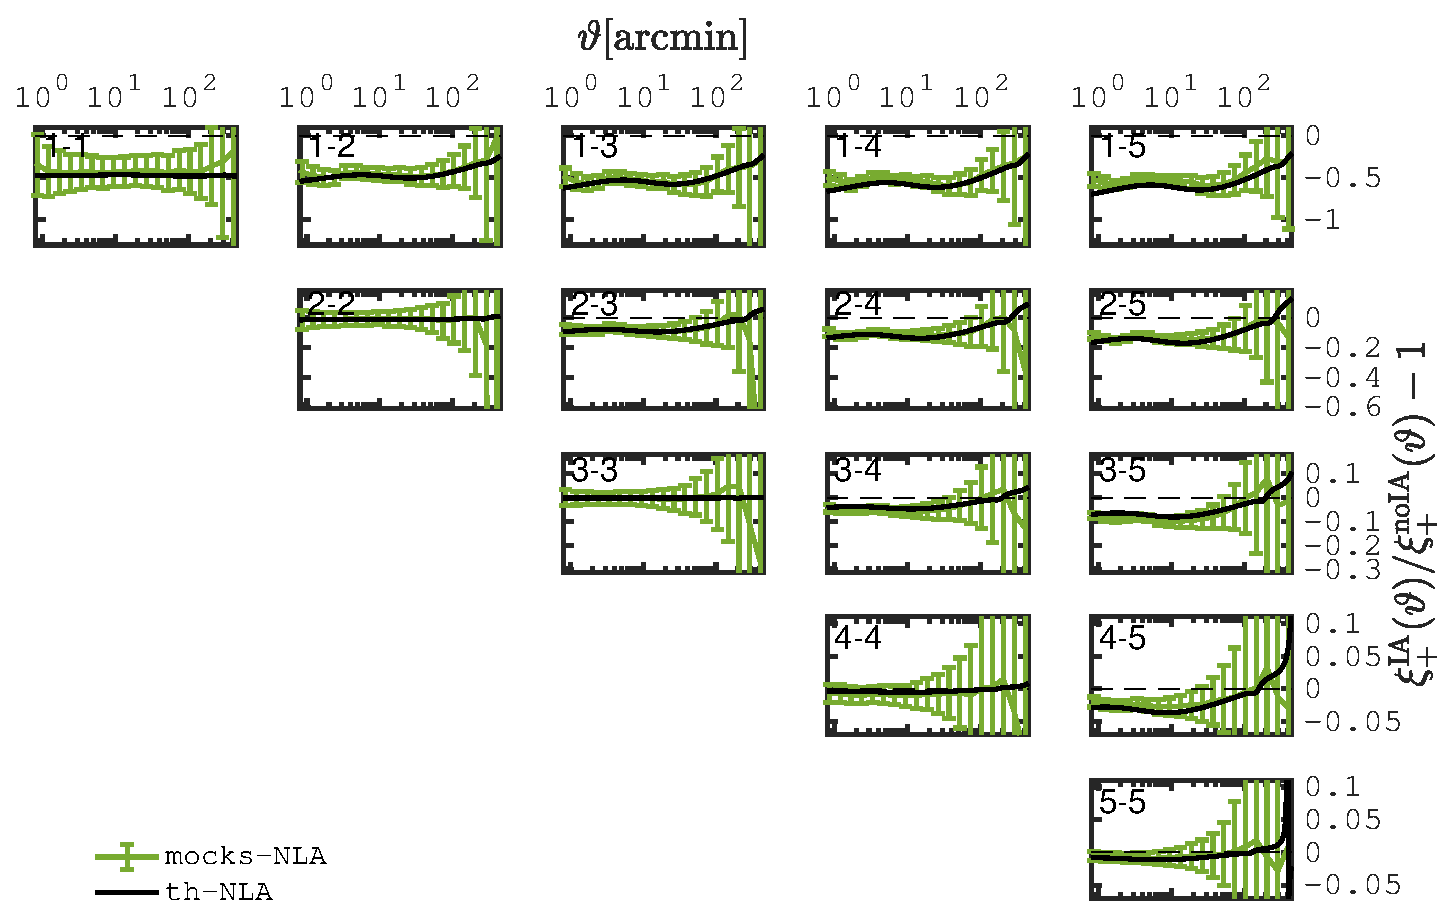
\includegraphics[width=\columnwidth]{graphs/frac_xip_IA1_skysim}
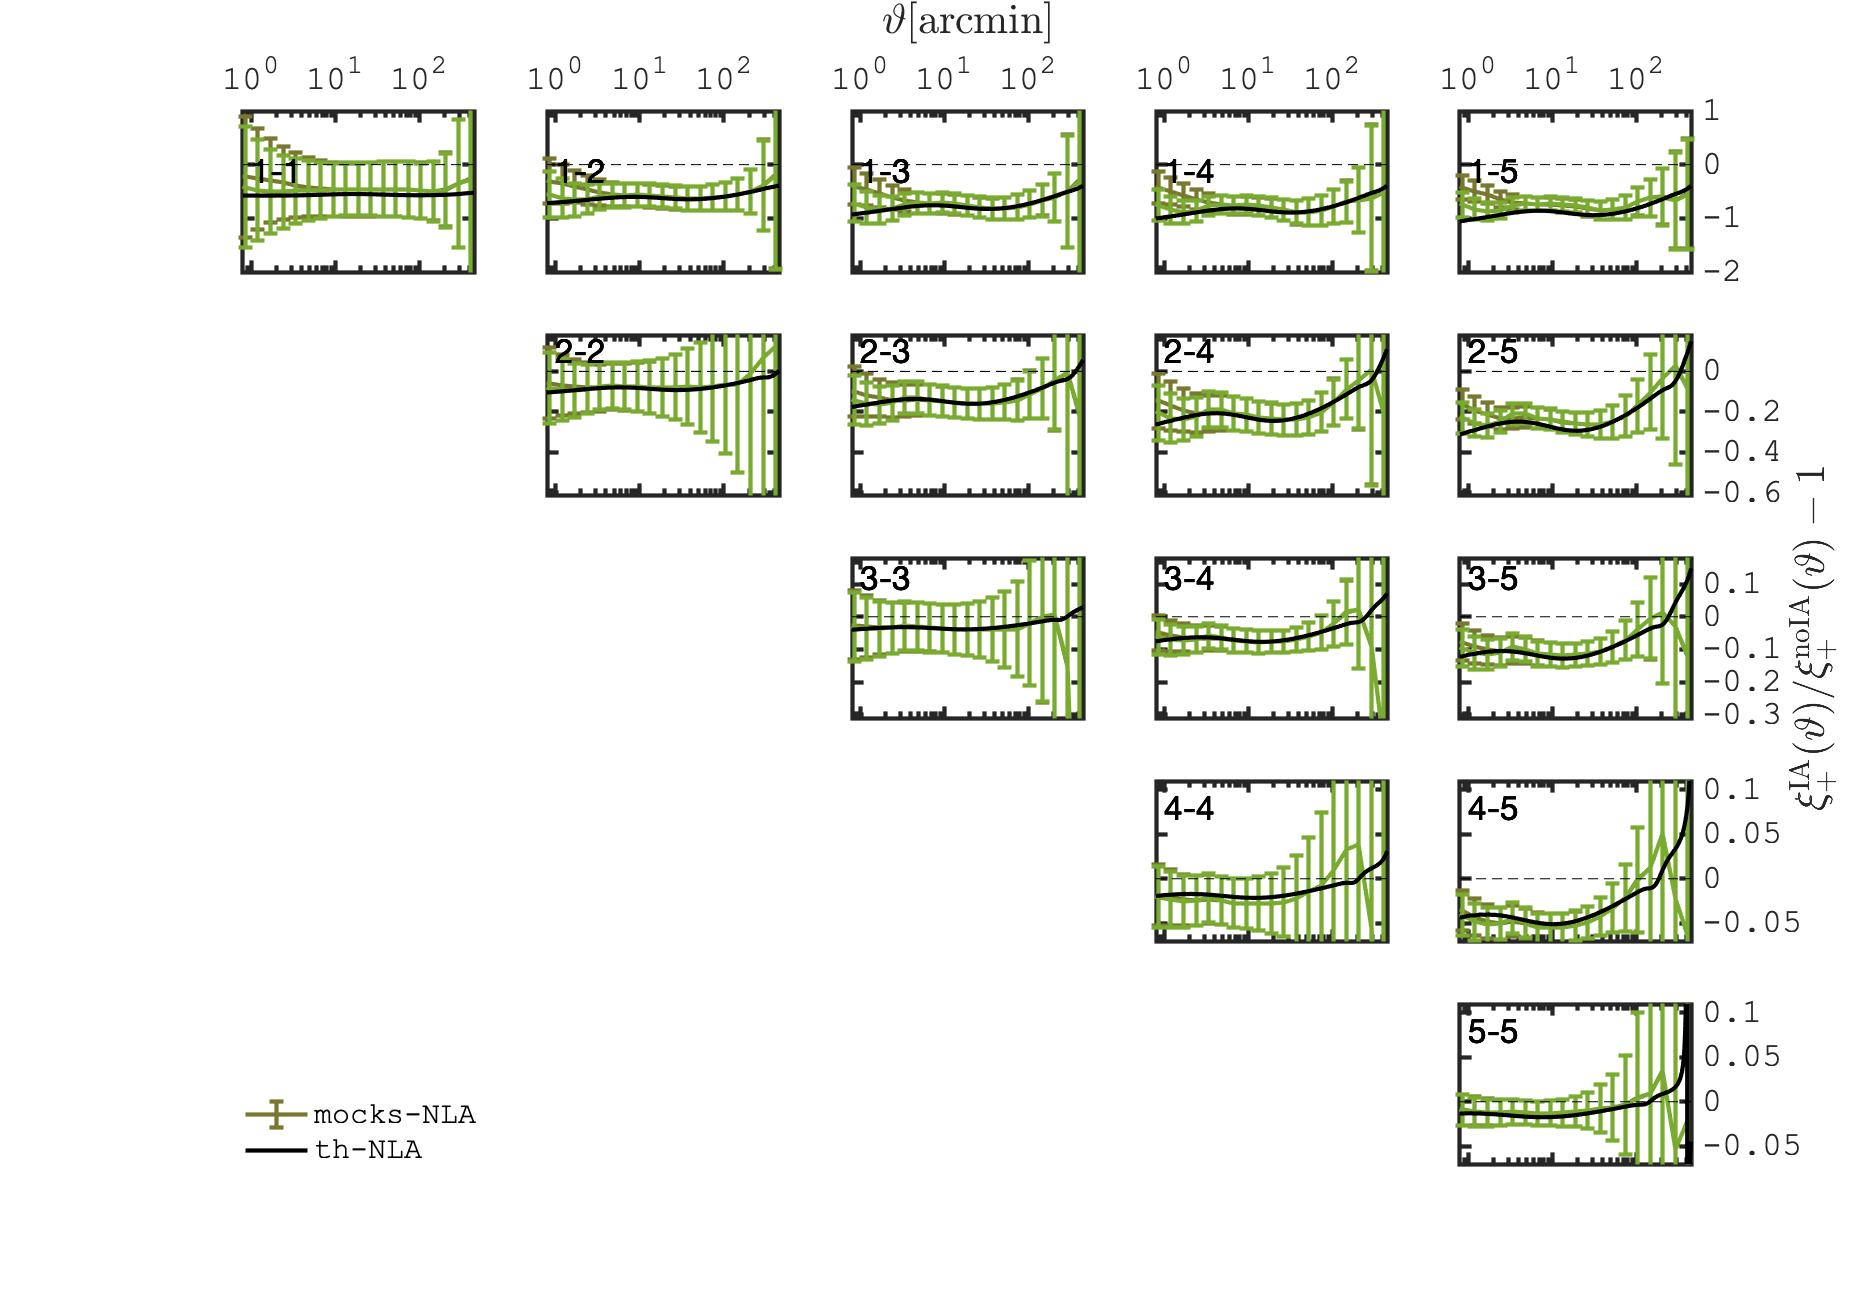
\includegraphics[width=\columnwidth]{graphs/frac_xip_IA1_skysim_NLA_srd.jpg}
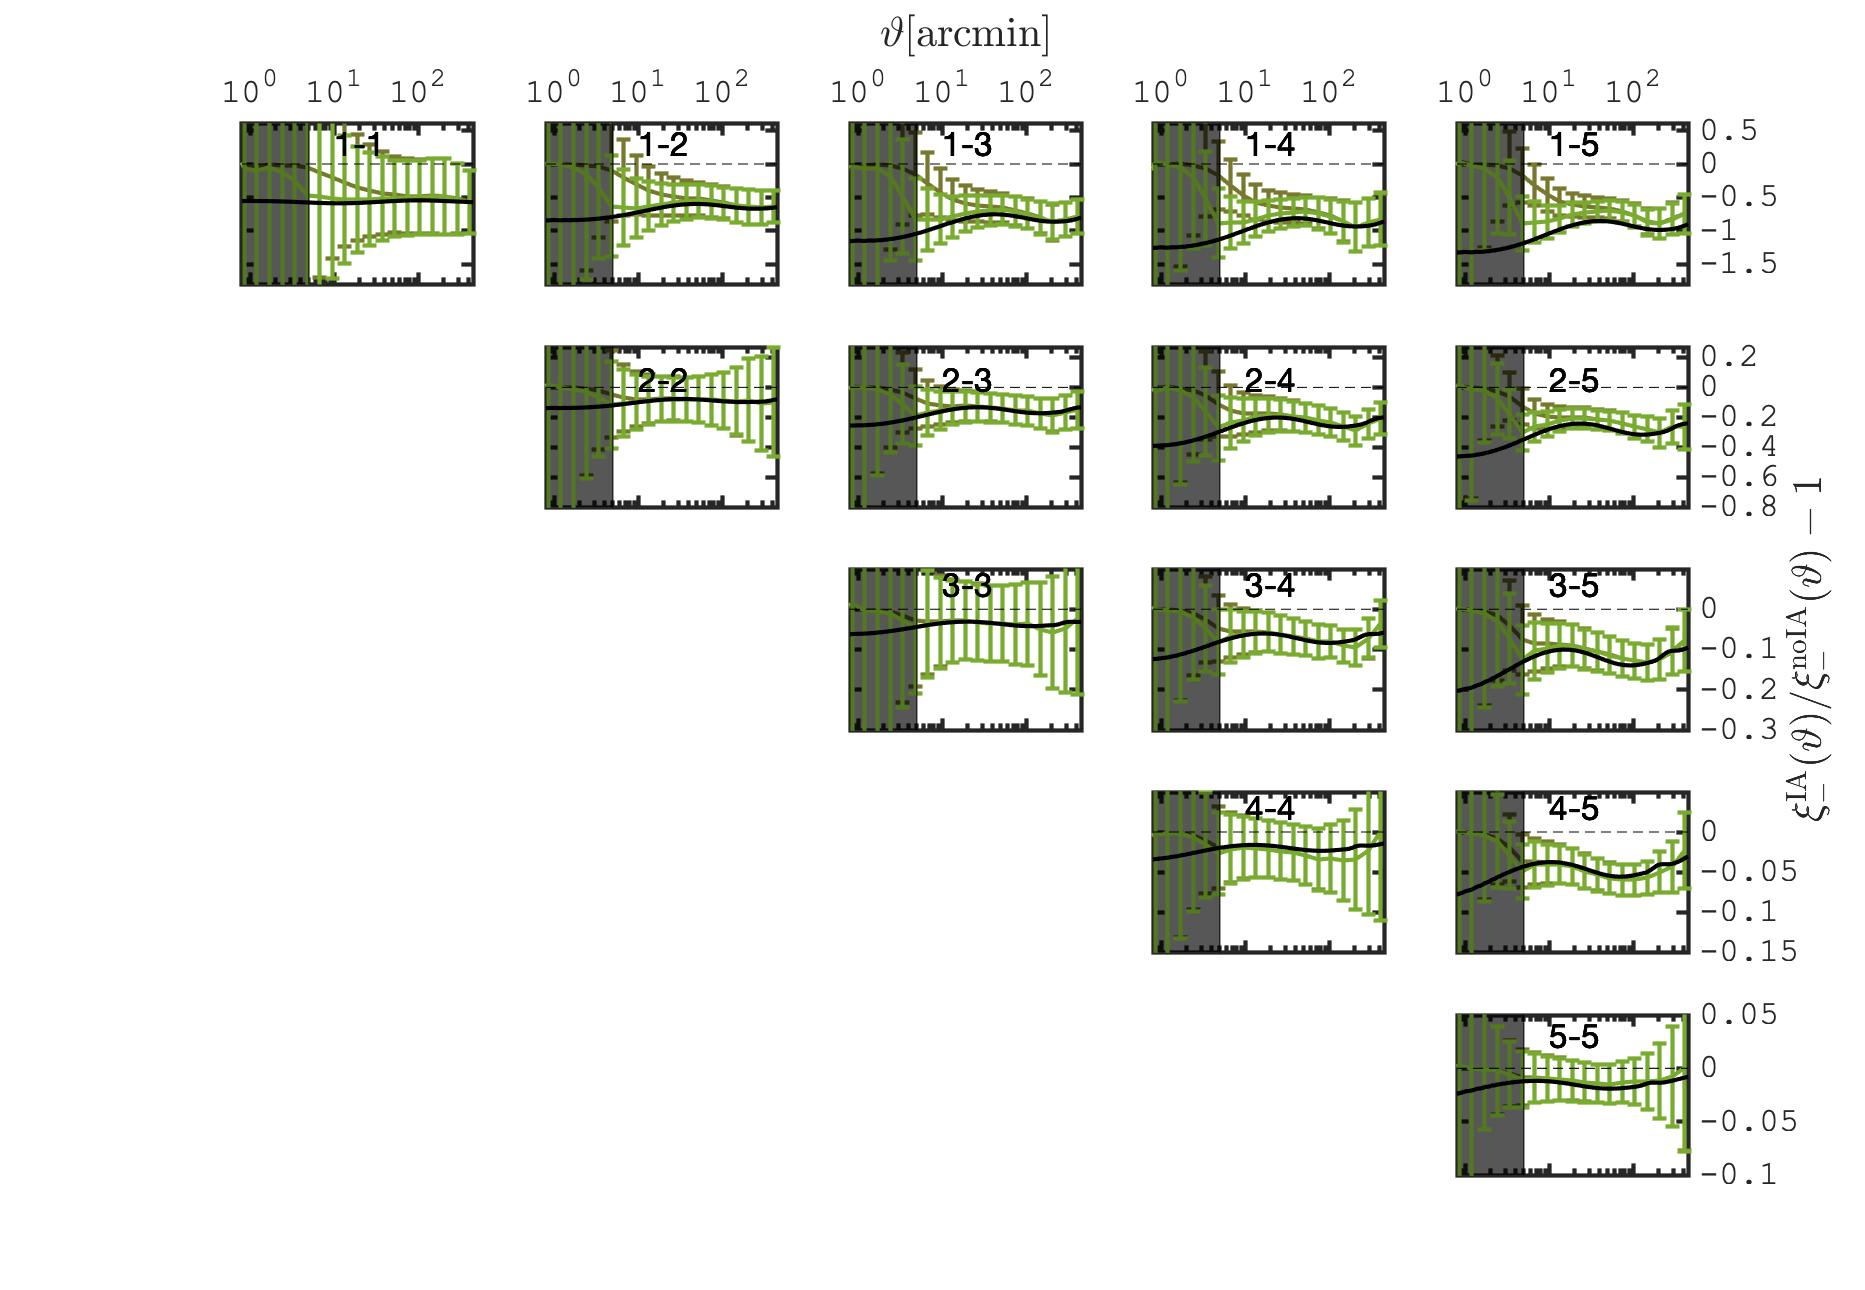
\includegraphics[width=\columnwidth]{graphs/frac_xim_IA1_skysim_NLA_srd.jpg}
\caption{Ratio between the shear correlation functions with and without IA, assuming the NLA model with $A_{\rm IA}=1.0$ both in the simulations and theory. Measurements shown in green and brown correspond to smoothing scales of 0.1 and 0.5 $h^{-1}$Mpc in the tidal field. There is no shape noise in the simulations, but it is included in the error bars.}
\label{fig:xi_NLA}
\end{figure*}
%---------------


\subsection{Data vector}
%------------------------------
\subsubsection*{NLA model}

We start by presenting a comparison between the relative impact of IA in the NLA model as measured in the simulations and as modelled by {\sc cosmoSIS}. Specifically, we show in Fig. \ref{fig:xi_NLA} the ratio between the $\gamma$-2PCF with and without IA, for all combinations of tomographic bins as indicated in the panels, and for two smoothing scales. The agreement is remarkable over all scales except for the smallest angular separations in $\xi_-$, where deviations are weaker in the simulations due to limits in the resolution.  The grey bands  indicates scales that are not well modelled and should be avoided, set to 5 arcmin. The smaller smoothing scales shows better agreement with the model at the smallest angular scales. 


%------------------------------
\subsubsection*{Extended-NLA model}
\begin{figure*}
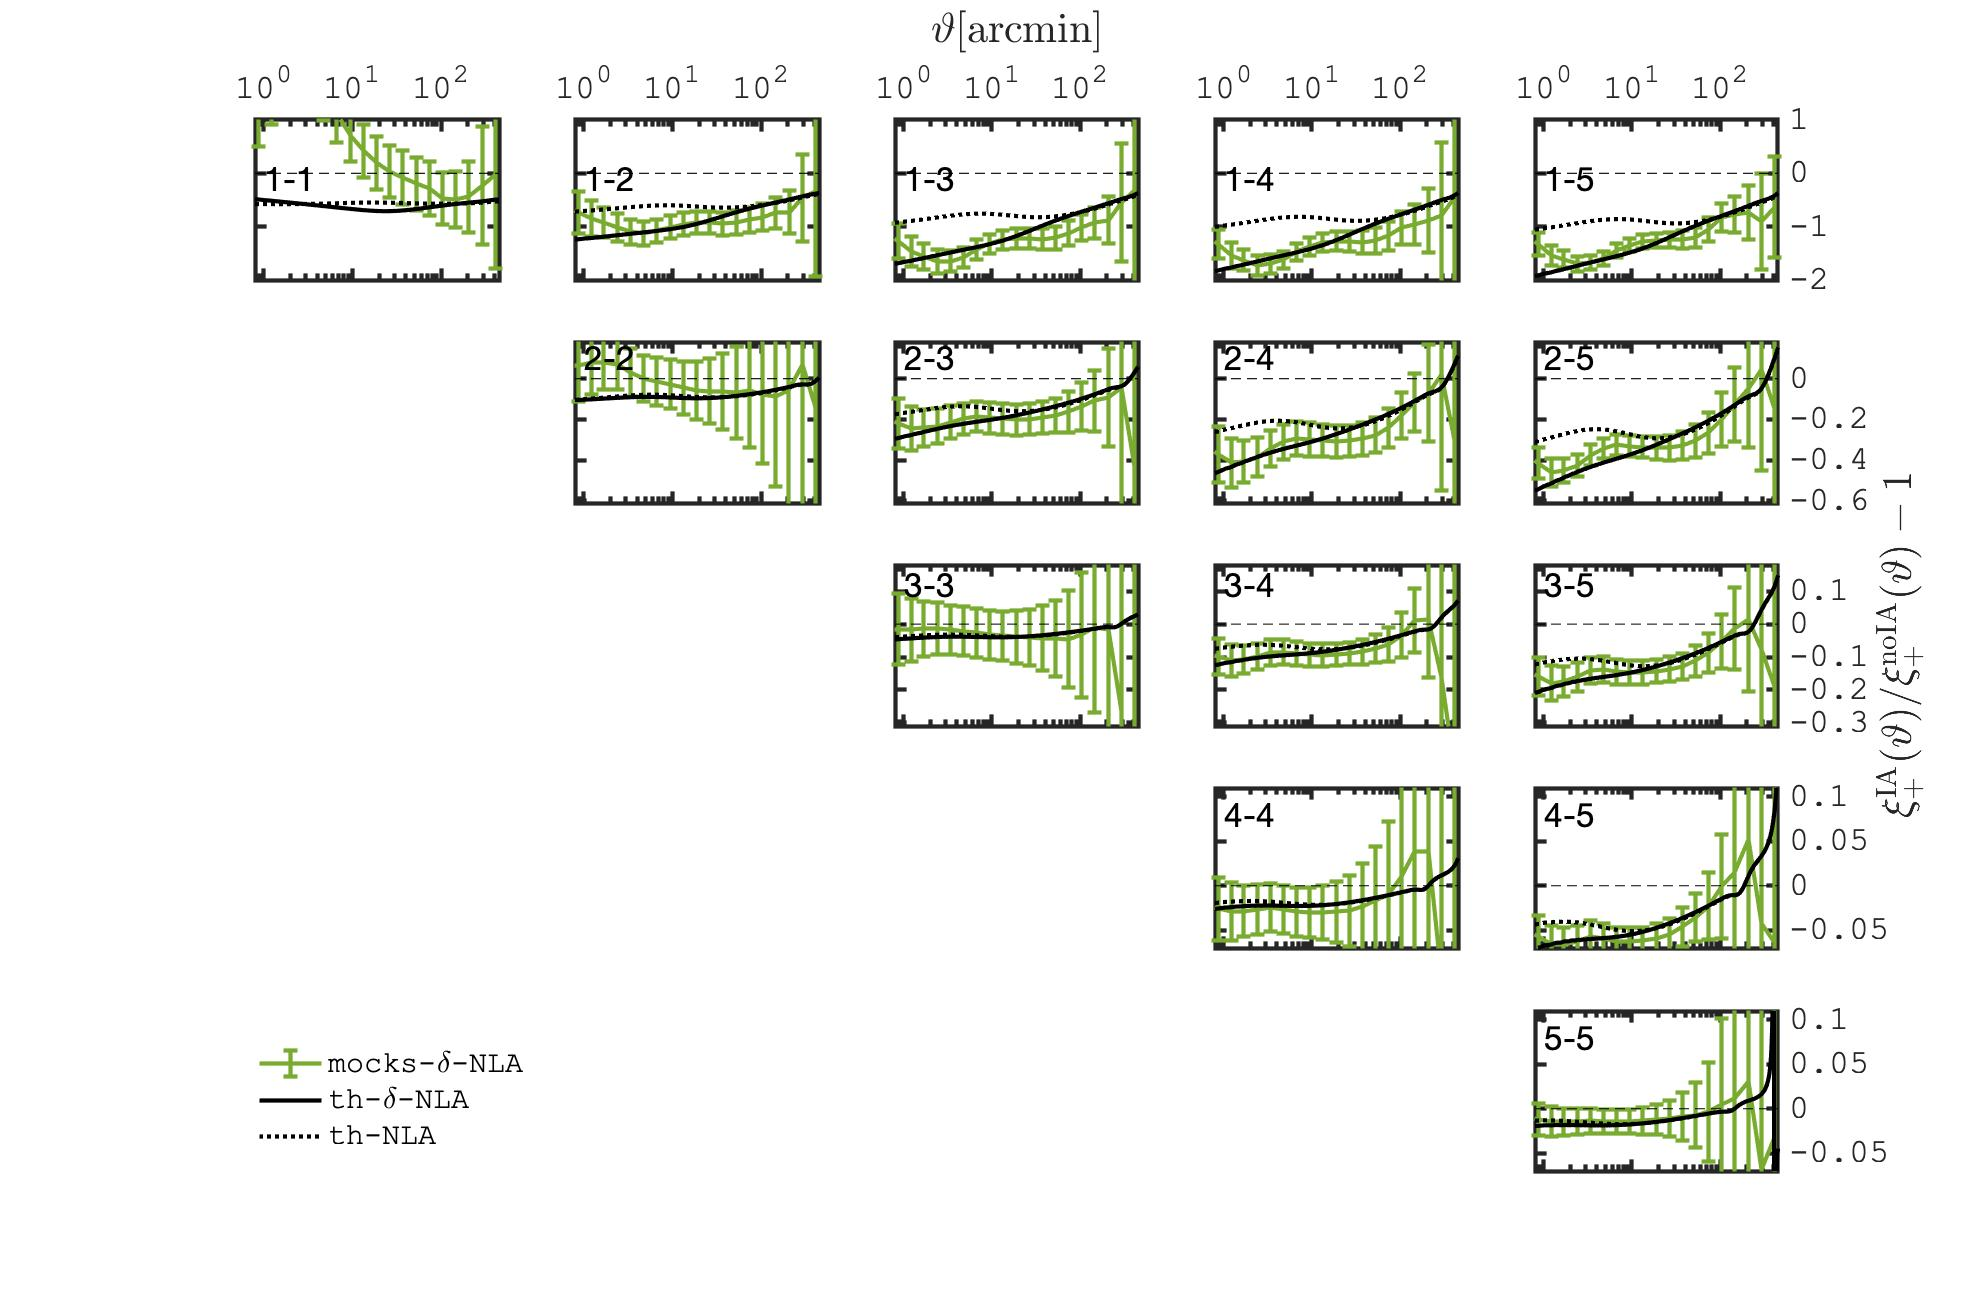
\includegraphics[width=\columnwidth]{graphs/frac_xip_IA1_skysim_deltaNLA_srd}
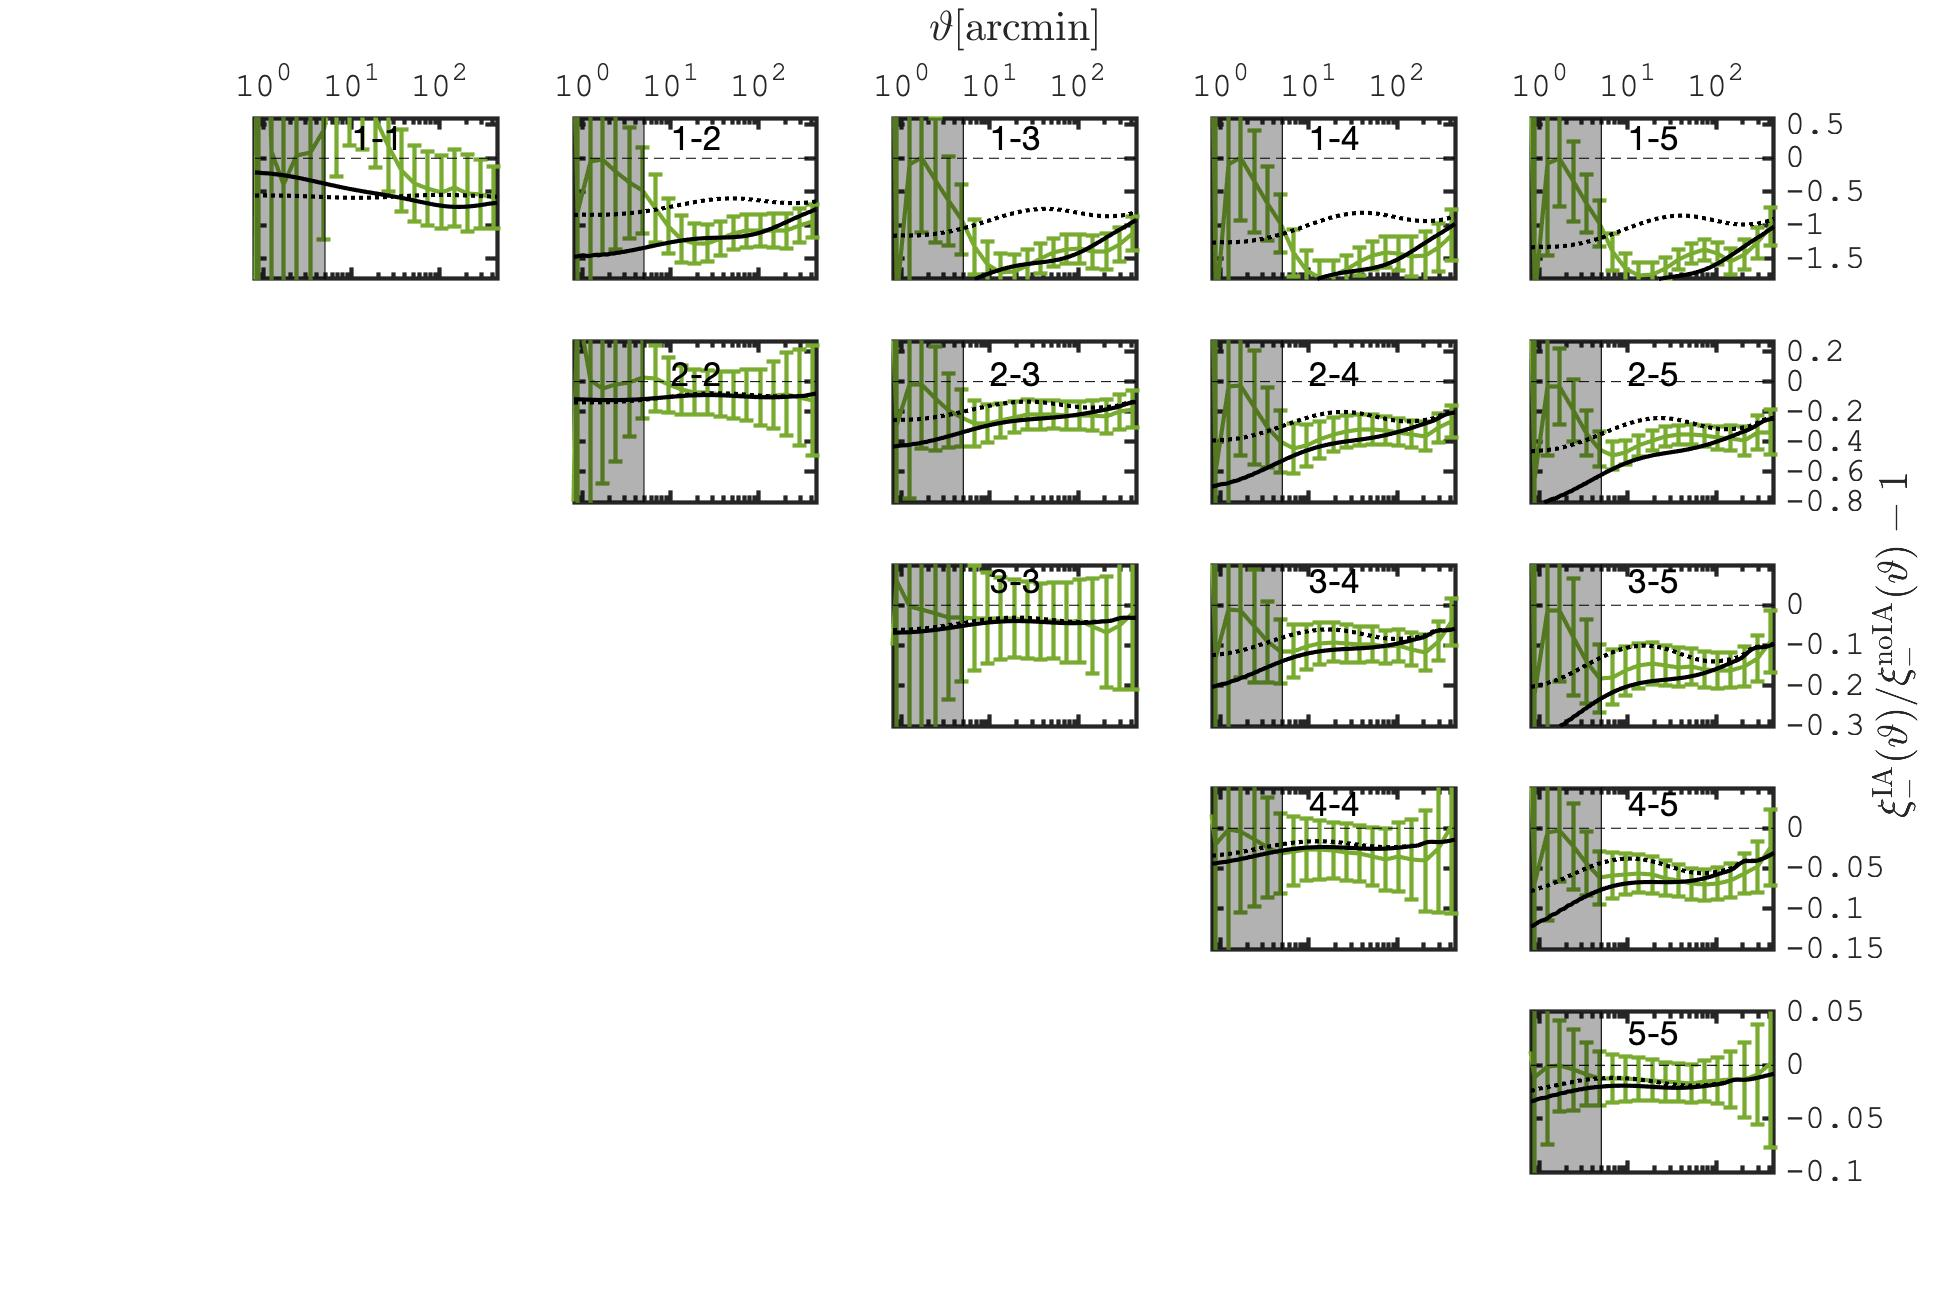
\includegraphics[width=\columnwidth]{graphs/frac_xim_IA1_skysim_deltaNLA_srd}
\caption{Same as Fig. \ref{fig:xi_NLA}, but for the $\delta$-NLA model with $A_{\rm IA}=1.0$ and $b_{\rm TA}=1.0$, and only for smoothing of 0.5$h^{-1}$Mpc. The dashed black lines show the NLA predictions to better highlight the differences.  }
\label{fig:xi_deltaNLA}
\end{figure*}

\begin{figure}
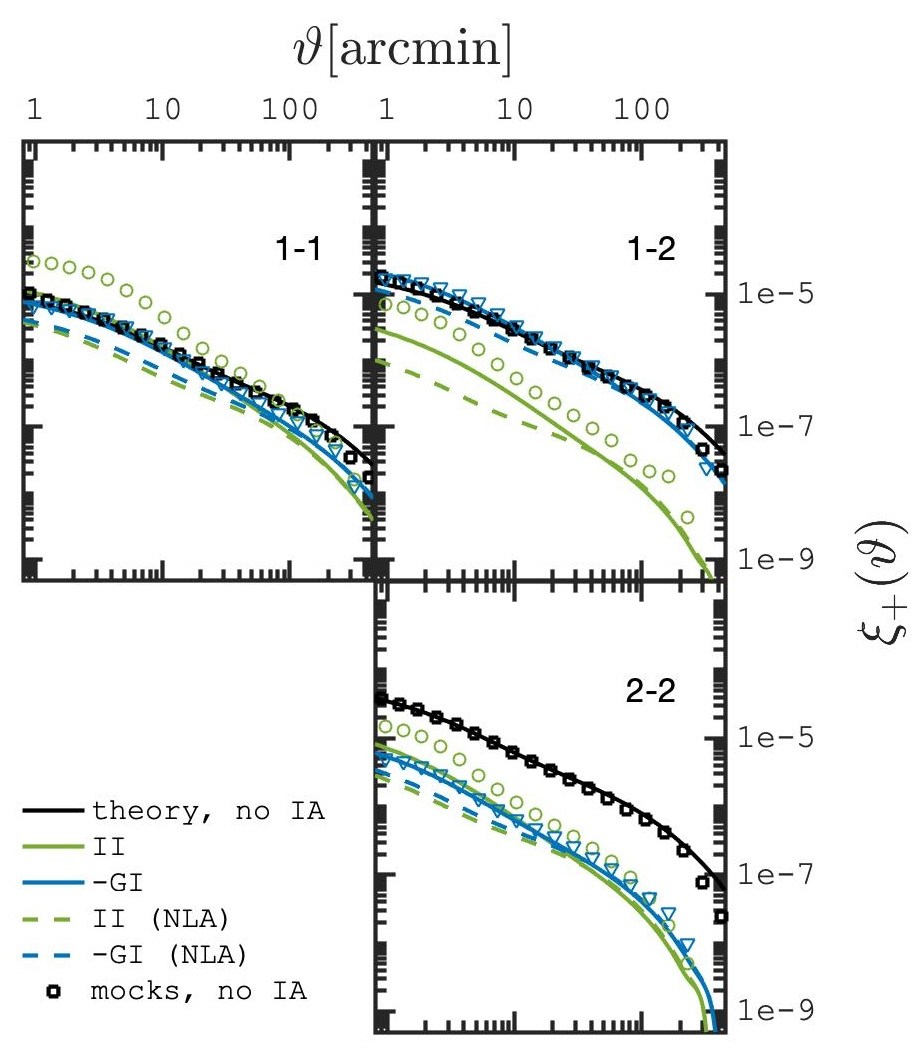
\includegraphics[width=\columnwidth]{graphs/xip_deltaNLA_bta1}
\caption{Shear 2PCF in the extended-NLA model for the two lowest redshift bins, showing the good agreement between simulations and theory for the $GG$ (black) and $GI$ (blue) terms, and large deviations in the $II$ term (green). {\it (Re-do legend)}}
\label{fig:xi_deltaNLA_II}
\end{figure}

\begin{figure}
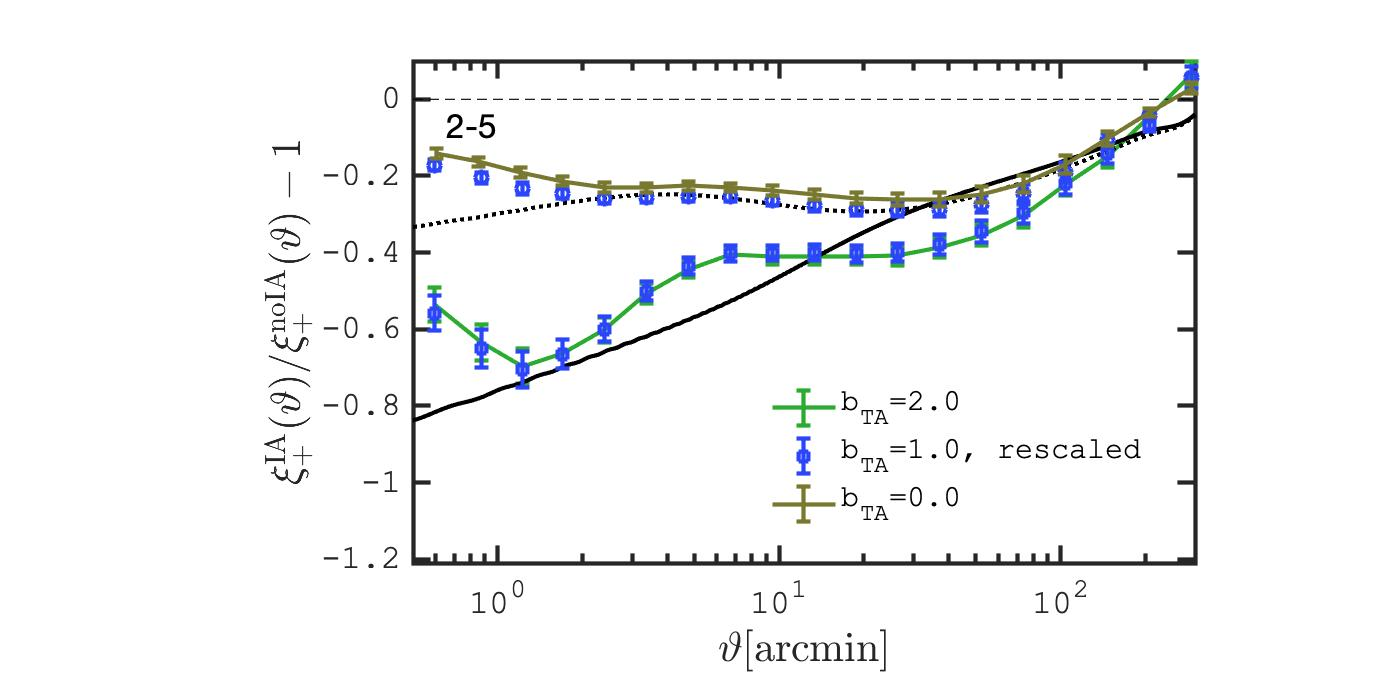
\includegraphics[width=\columnwidth]{graphs/frac_xip_bta1_rescaled}
\caption{Ratio between the shear correlation functions with and without IA in tomographic bin combination 2-5.
The brown and green symbols show measurements from simulations constructed with $b_{\rm TA}$ = 0.0 and 2.0 respectively,  the black solid and dotted lines shown their predictions, while the blue symbols are obtained by rescaling $b_{\rm TA}$ = 1.0 simulations using Eq. \ref{eq:bta_rescale}.  }
\label{fig:xi_deltaNLA_rescaled}
\end{figure}

The equivalent comparison for the extended-NLA model is presented in Fig. \ref{fig:xi_deltaNLA}, where we also find an excellent match with the theoretical predictions except for redshift bins 1-1 and 2-2, where the $II$ term is important and much larger in the simulations than in the theory. This is expected since the former includes additional terms that are up to second order in perturbation theory. This is shown in Fig. \ref{fig:xi_deltaNLA_II}, where the different contributions are separated, clearly showing the disagreement in  the $II$ term. 

The results are shown here for $b_{\rm TA}$ = 1.0  and we verified that it works equally well for $b_{\rm TA}$ =  2.0. Using the former, we test the $b_{\rm TA}$-rescaling method introduced in Eq. \ref{eq:bta_rescale} to generate $b_{\rm TA}=2.0$ and $b_{\rm TA}=0.0$ mocks, and compare the outcome with mocks constructed directly with these bias values. Results are shown in Fig. \ref{fig:xi_deltaNLA_rescaled} for one of the tomographic bins for which IA has the strongest effect. The match is excellent here, however lower redshift are less accurate due to the increased shot noise (not shown){\it (should I show an example?)}, hence we recommend producing new mocks over using this rescaling method whenever possible. 

Note that since source clustering is a higher order effect in cosmic shear, the measured $\xi_{\pm}$ from mocks with $b_{\rm TA}$=0.0, 1.0 and 2.0 show negligible differences in $\xi_+$, and becomes detectable only at the smallest scales  (i.e. $\vartheta<5$arcmin) in $\xi_-$, consistent with  \citet{source_lens_clustering} who find an effect of a few percent for $\ell>3000$, and with \citet{DESY3_Gatti_source_clust}, who find minor impact for second moments of aperture mass maps. However the impact on higher order lensing statistics and on the overall  IA contamination is significant and can double the secondary signal in certain circumstances, due to the up-sampling of regions with strong tidal forces. 

% Requires the booktabs if the memoir class is not being used
\begin{table}
   \centering
   %\topcaption{Table captions are better up top} % requires the topcapt package
    \caption{IA models infused in this work and the respective fiducial values of the model parameters.}
   \begin{tabular}{@{} lcr @{}} % Column formatting, @{} suppresses leading/trailing space
      \hline
      \hline
      %\multicolumn{2}{c}{Item} \\
      model   		& ($A_{\rm IA}, \: b_{\rm TA}, \: A_2)$ \\
      \hline
      NLA     		& ($\pm$1, 0, 0) &  \\
      \hline
      \multirow{2}{*}{extended-NLA }  	&   ($\pm$1, 1, 0)   \\
                                        &  (1, 2, 0)   \\
      \hline
      TT 			&  {(0, 0, $\pm$1)} &  \\
      \hline
      \multirow{2}{*}{extended-TT} 	    &  (0, 1 ,$\pm$1)   \\
                                        &  (0, 2, 1)   \\
      \hline
      TATT- fiducial	&  (1, 1, 1)  \\
      \hline
      \hline
   \end{tabular}
   \label{table:IAmodels}
\end{table}





%------------------------------


%------------------------------
\subsubsection*{TT model}
\label{subsec:TT}

Results for the tidal torque model are presented in Fig. \ref{fig:xi_TT}, again for two smoothing scales. In this case, we see that the larger smoothing scales agrees better with the theoretical predictions, likely due a mis-matched caused by projection effects. Indeed, the TT model, being quadratic in the tidal field, is more sensitive to smaller scales \citep{TATT}, and the missing third dimension inherent to our method is more prone to cause inaccuracies. We observe discrepancies in the small angular separations for  $\xi_-$ at low redshifts, but achieve better match for $\vartheta>$  40 arcmin.

Importantly, we found that our implementation of the TT model yields alignments that are too strong at low redshifts, and hence requires an empirical redshift-dependent calibration to improve the match with theory. We achieve this by rescaling $\epsilon^{\rm IA, TT}(z<0.5) \rightarrow \epsilon^{\rm IA, TT} /2.5$, acknowledging that this exhibits limits in our capacity to model the tidal torquing without accessing the third dimensional of the tidal field. 

\begin{figure*}
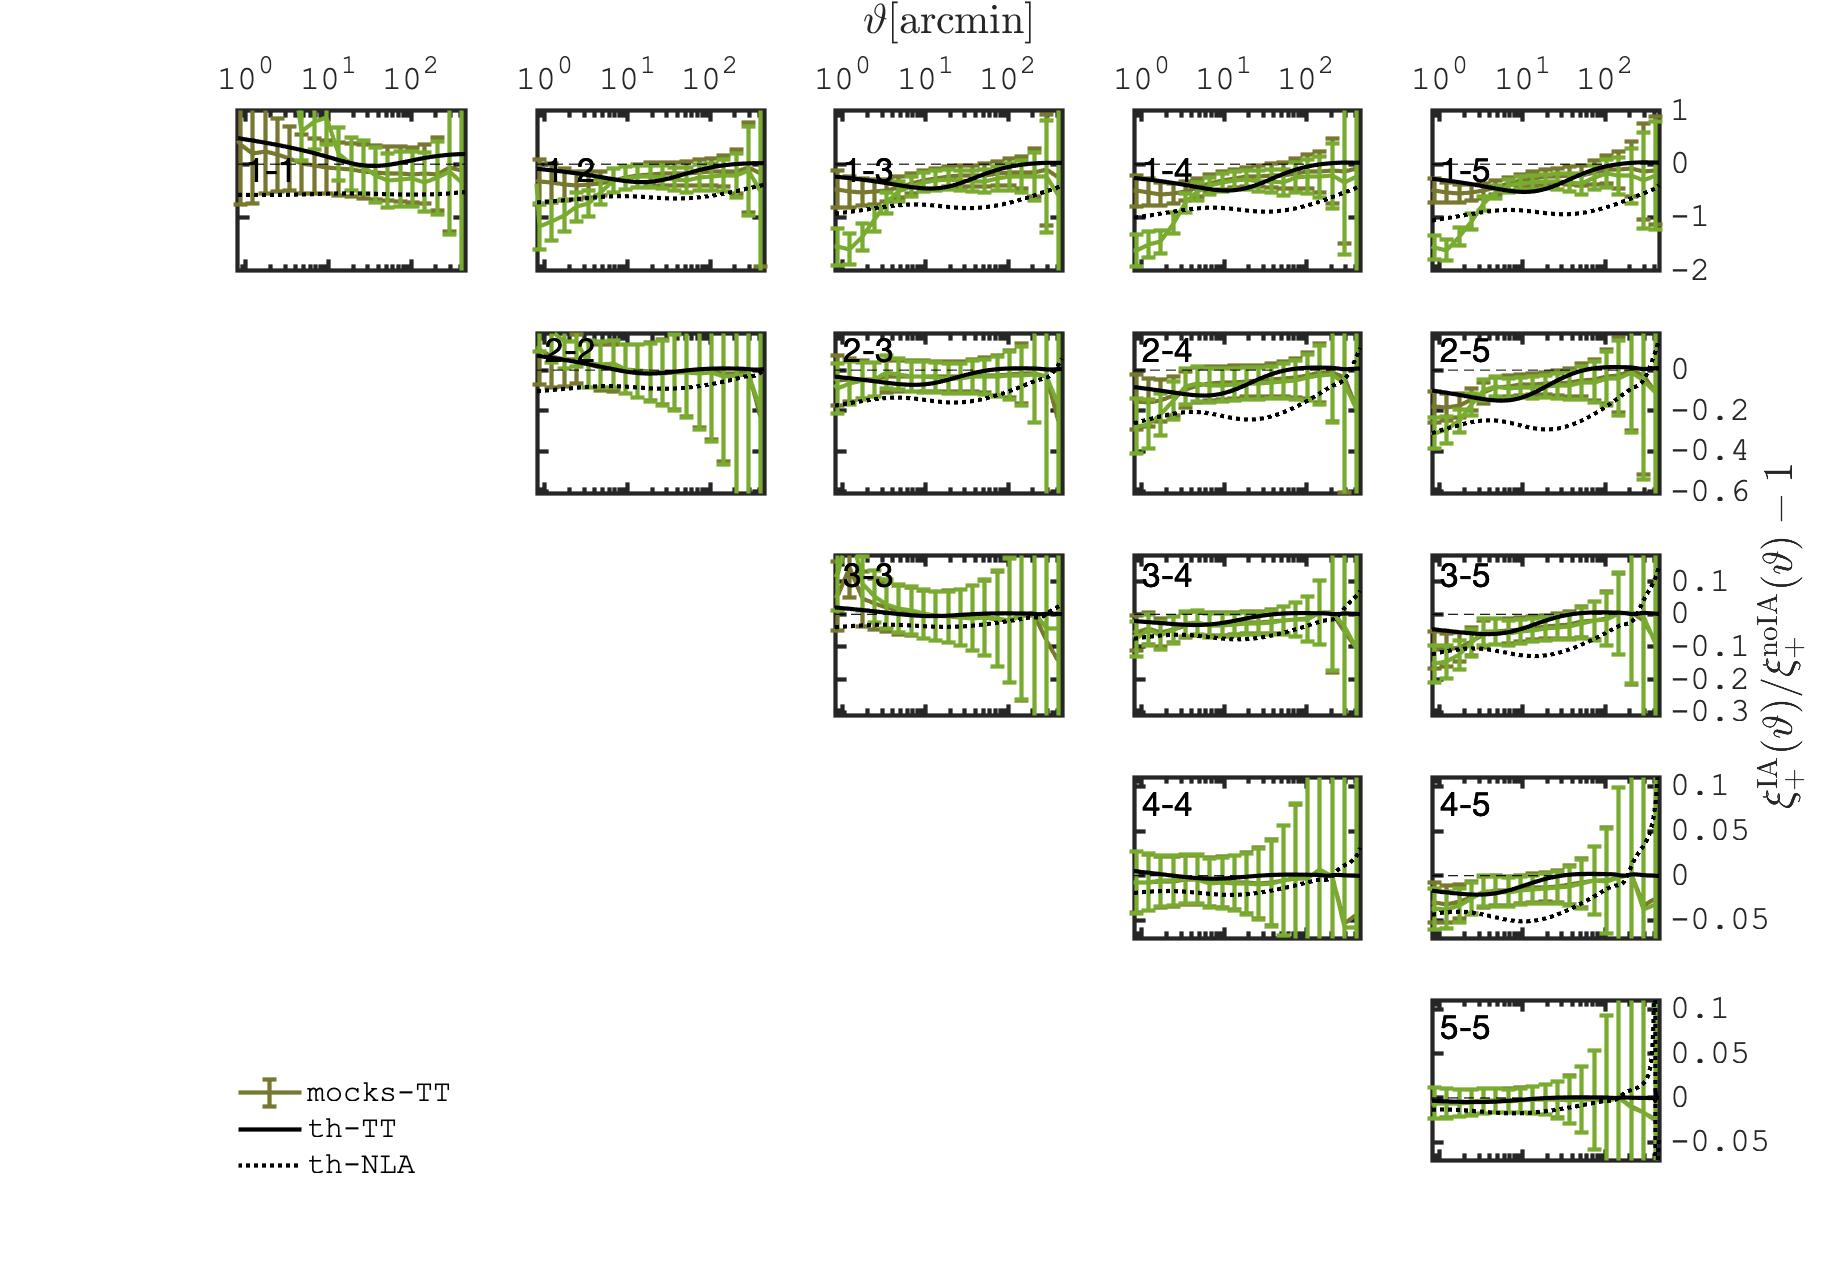
\includegraphics[width=\columnwidth]{graphs/frac_xip_IA1_skysim_TT_srd.jpg}
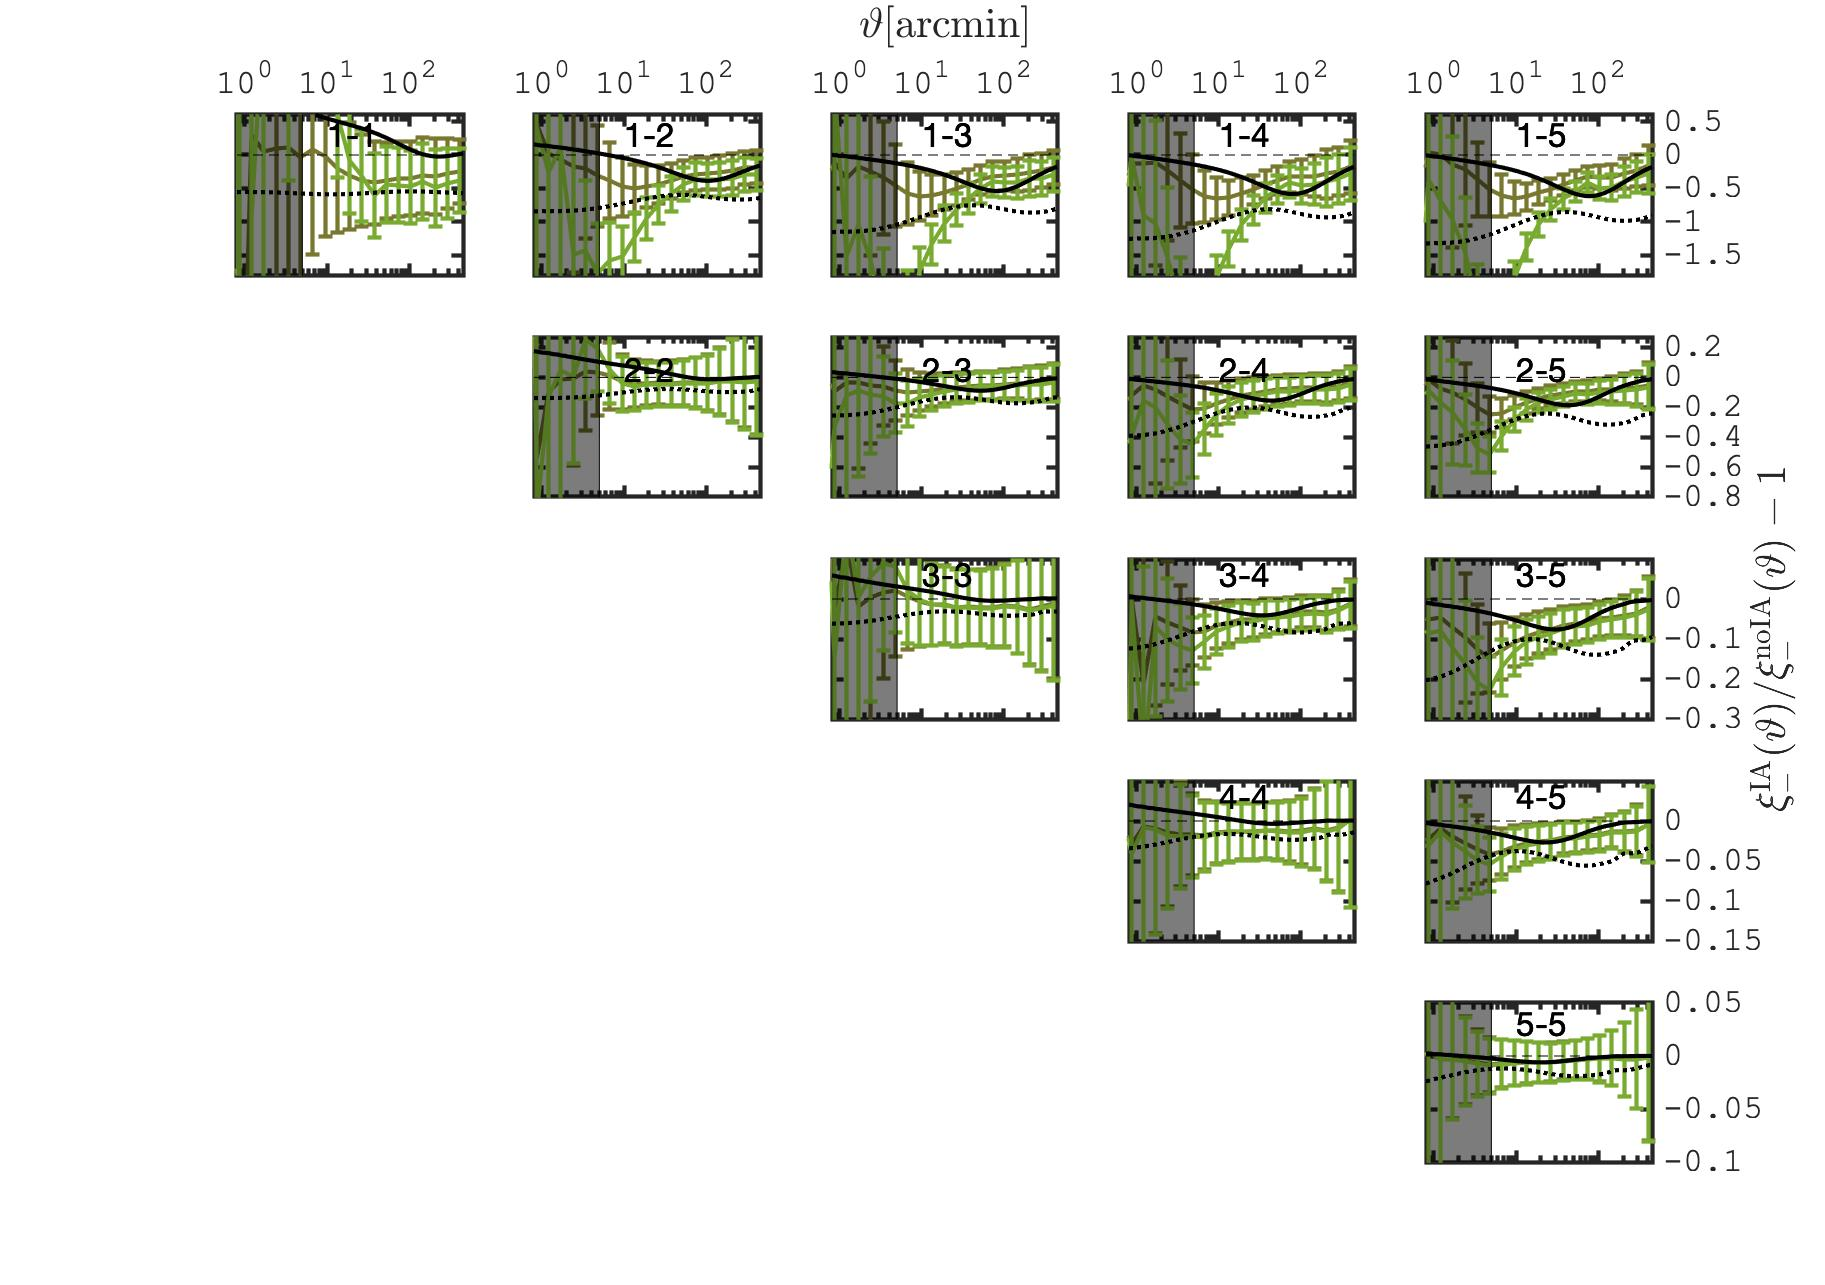
\includegraphics[width=\columnwidth]{graphs/frac_xim_IA1_skysim_TT_srd.jpg}
\caption{Same as Fig. \ref{fig:xi_NLA}, but for the TT model with $A_2=1.0$. Brown is smoothing scale of 0.5 arcmin, green is 0.1 arcmin. Here, the dashed black lines show the NLA predictions to better highlight the differences. }
\label{fig:xi_TT}
\end{figure*}

\begin{figure*}
%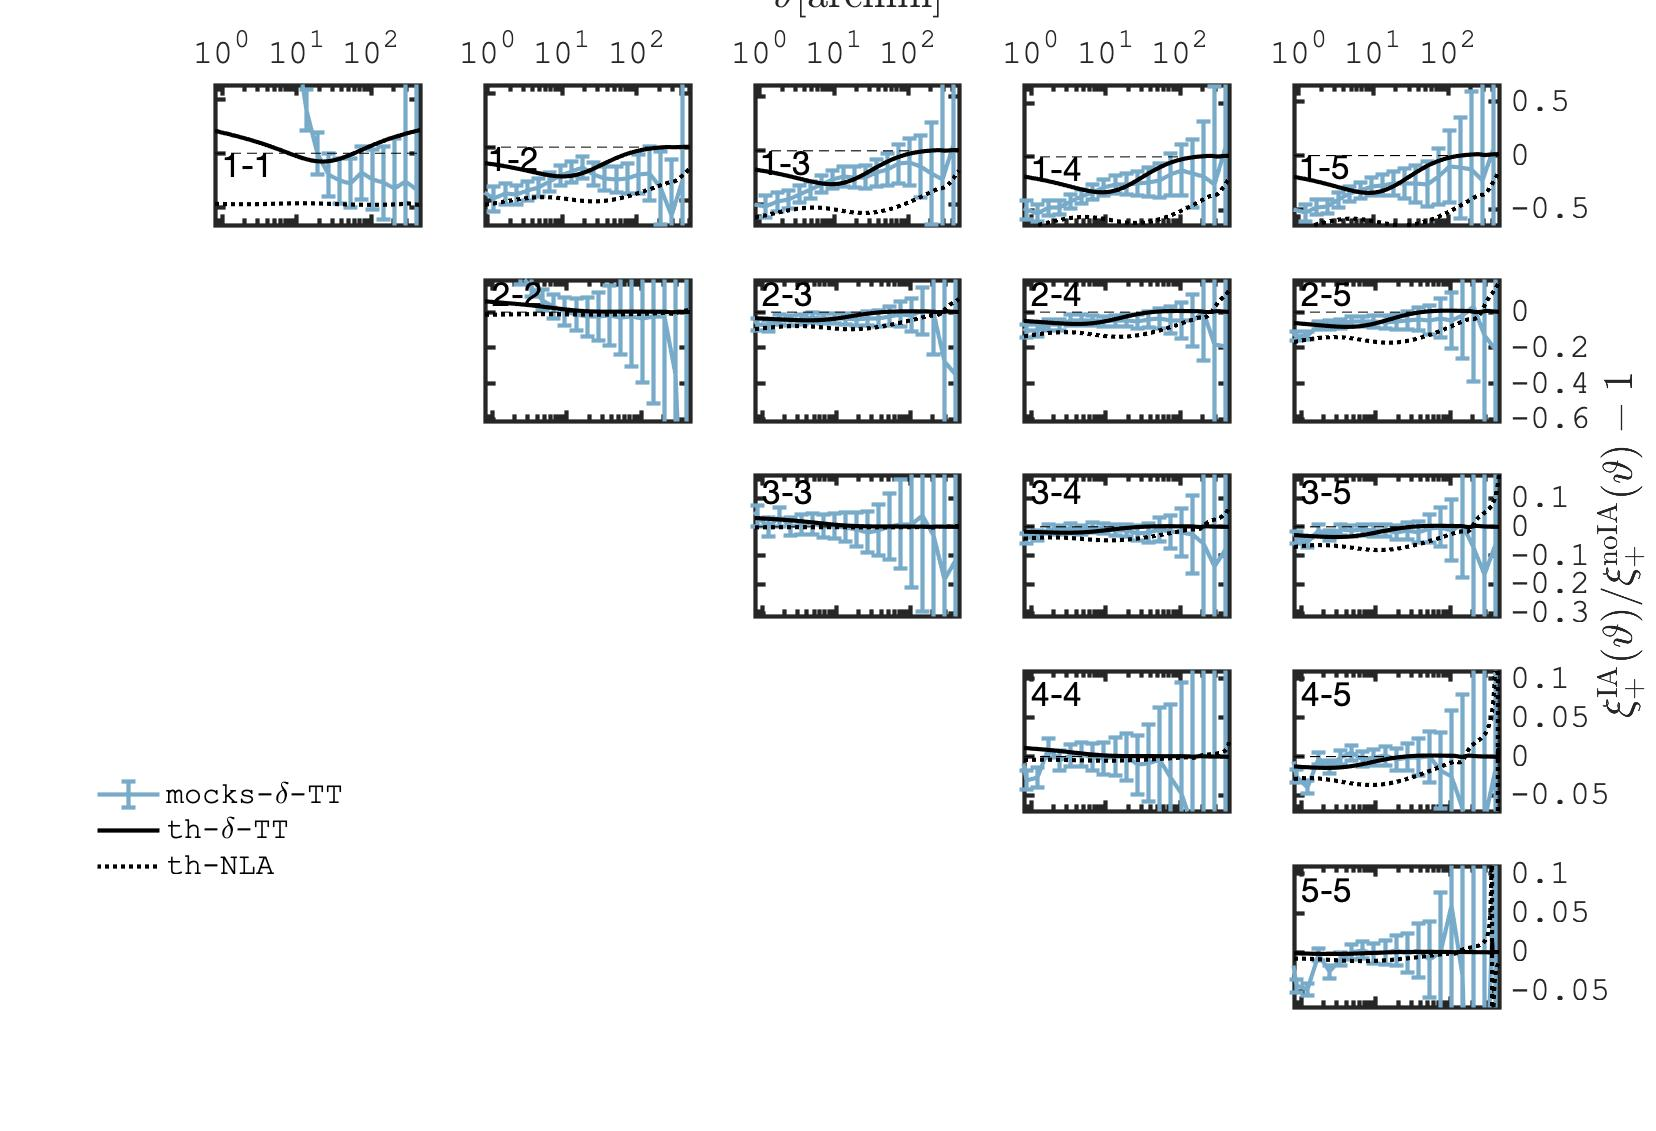
\includegraphics[width=\columnwidth]{graphs/frac_xip_C2_m1_skysim_deltaTT}
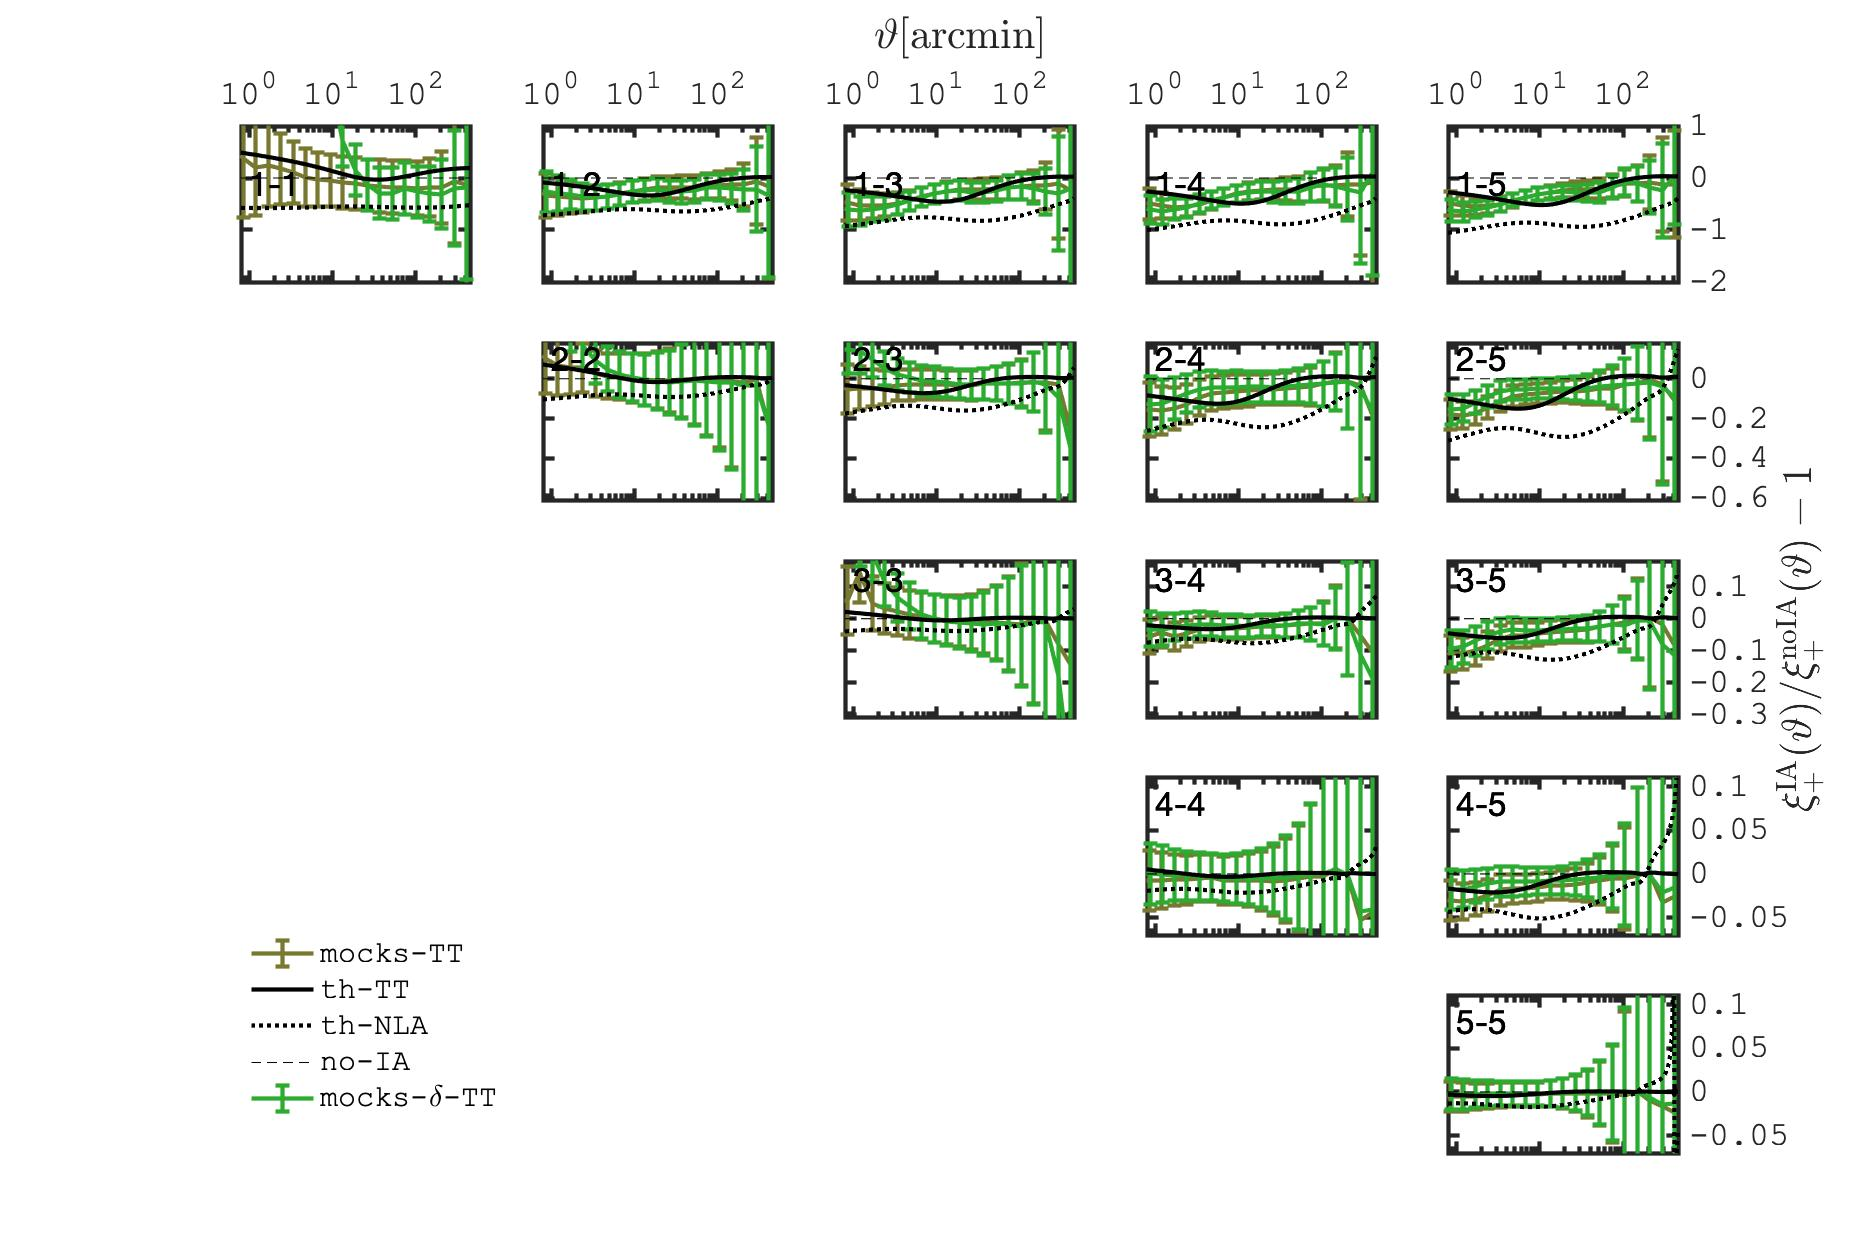
\includegraphics[width=\columnwidth]{graphs/frac_xip_IA1_skysim_deltaTT_srd.jpg}
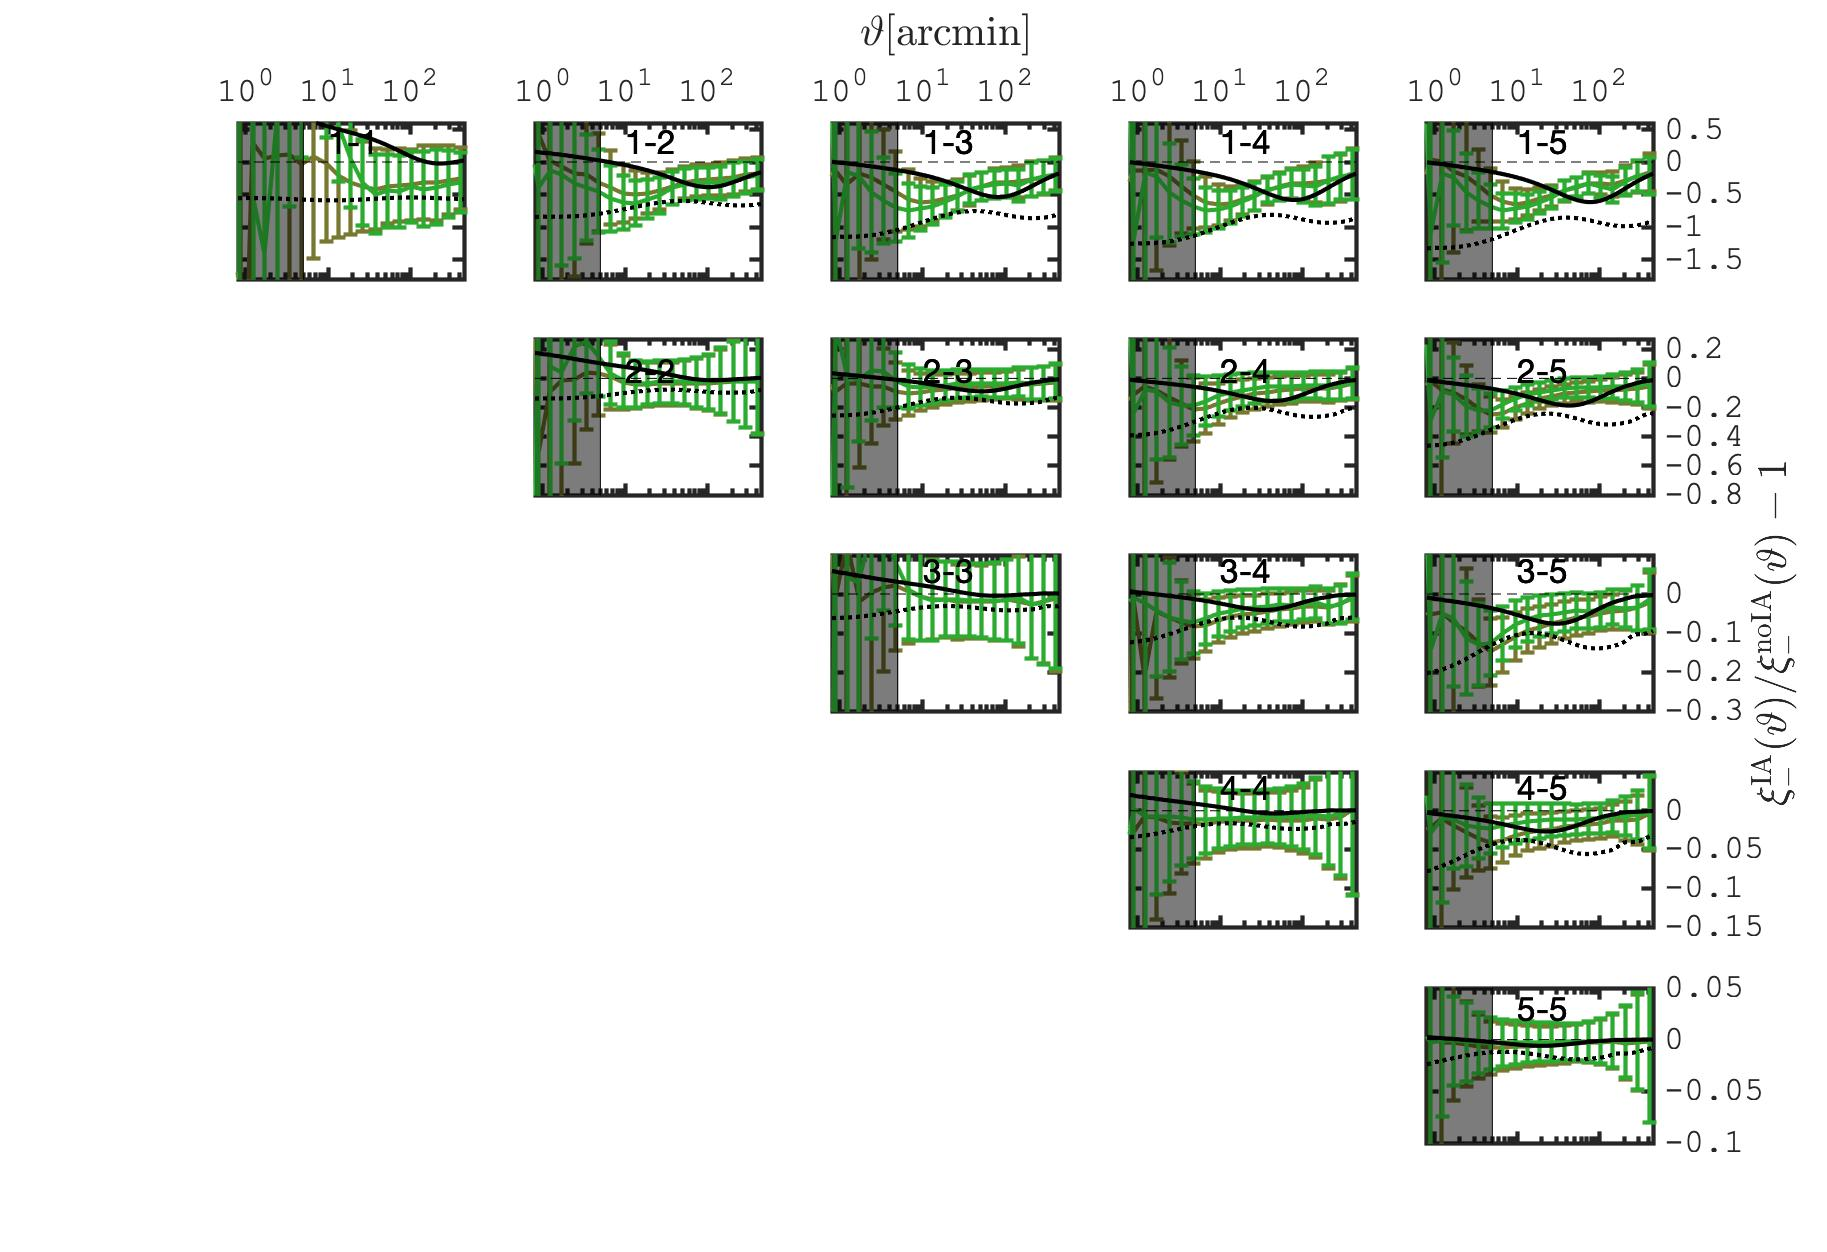
\includegraphics[width=\columnwidth]{graphs/frac_xim_IA1_skysim_deltaTT_srd.jpg}
\caption{Same as Fig. \ref{fig:xi_deltaNLA}, but comparing the TT (brown) and the $\delta$-TT  (green) models, with $A_2=1.0$, $b_{\rm TA}$ = 1.0, and only for smoothing of 0.5$h^{-1}$Mpc. }
\label{fig:xi_deltaTT}
\end{figure*}



%------------------------------
\subsubsection*{Extended-TT model}
\label{subsec:TT}

The extended-TT model, constructed by using the TT coupling on galaxies linearly tracing the underlying matter density, also needs to be calibrated. This has some degree of arbitrariness due to the absence of theoretical model to match it against. We choose to match the TT theory on large angular separation at all redshifts, physically motivated from the fact that this modified galaxy bias should not impact strongly scales that are much larger than galaxy clusters.
This therefore required us to lower the original ellipticities, especially at low $z$: $\epsilon^{{\rm IA}, \delta{\rm TT}}(z<0.5) \rightarrow \epsilon^{{\rm IA}, \delta{\rm TT}} /2.5$ as for the normal TT model, further followed by a global $\epsilon^{{\rm IA}, \delta{\rm TT}} \rightarrow \epsilon^{{\rm IA}, \delta{\rm TT}}/20.0$ rescaling. This is a large calibration condition, which compensate for the overly strong coupling computed from our simulations. The results are shown in Fig. \ref{fig:xi_deltaTT}, where we observed that the deviations with respect to the TT model occur at small angular scales ($\vartheta < $ 20 arcmin) in $\xi_+$, and for the lowest redshifts. Although this model is harder to match with current theoretical IA model, it provides a good example with which we can study the impact of IA mis-modelling, e.g. analysing this model with the TATT predictions, similar to the investigations of \citet{Paopiamsap2024}.


%------------------------------
\subsubsection*{HOD-TATT model}
\label{subsec:HOD}


%--------------
\begin{figure*}
%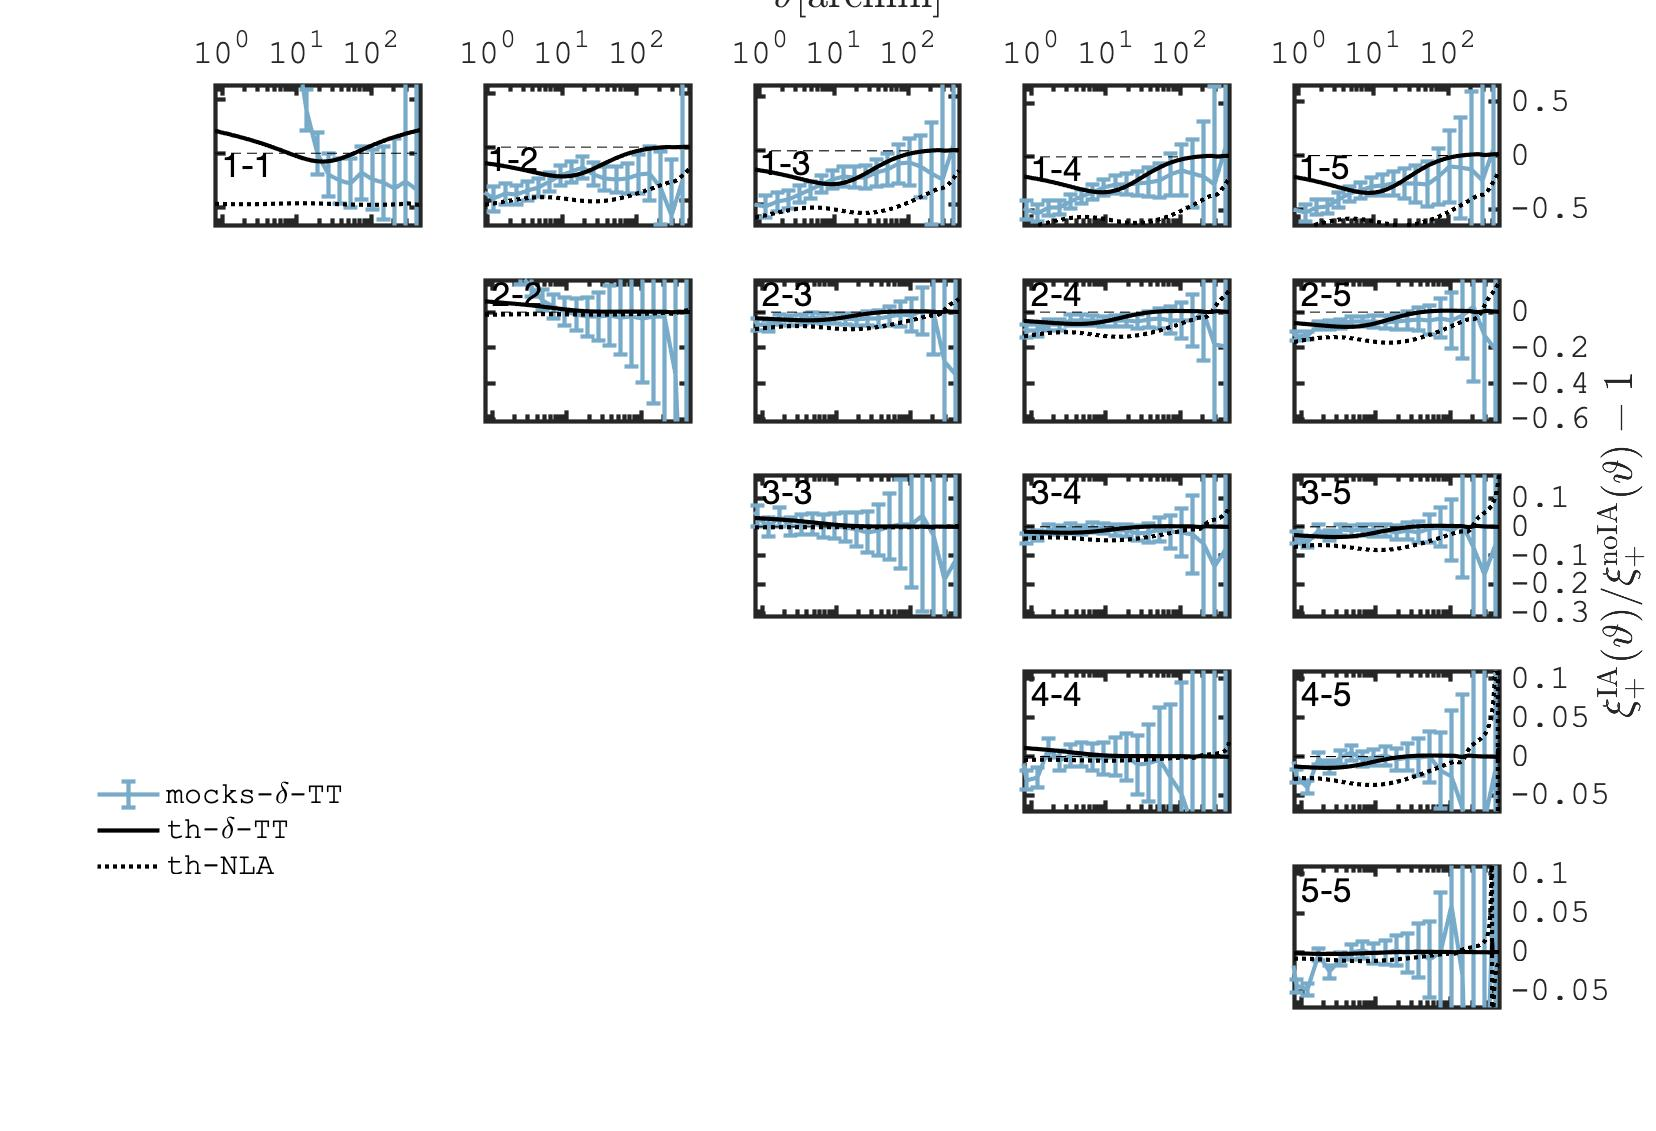
\includegraphics[width=\columnwidth]{graphs/frac_xip_C2_m1_skysim_deltaTT}
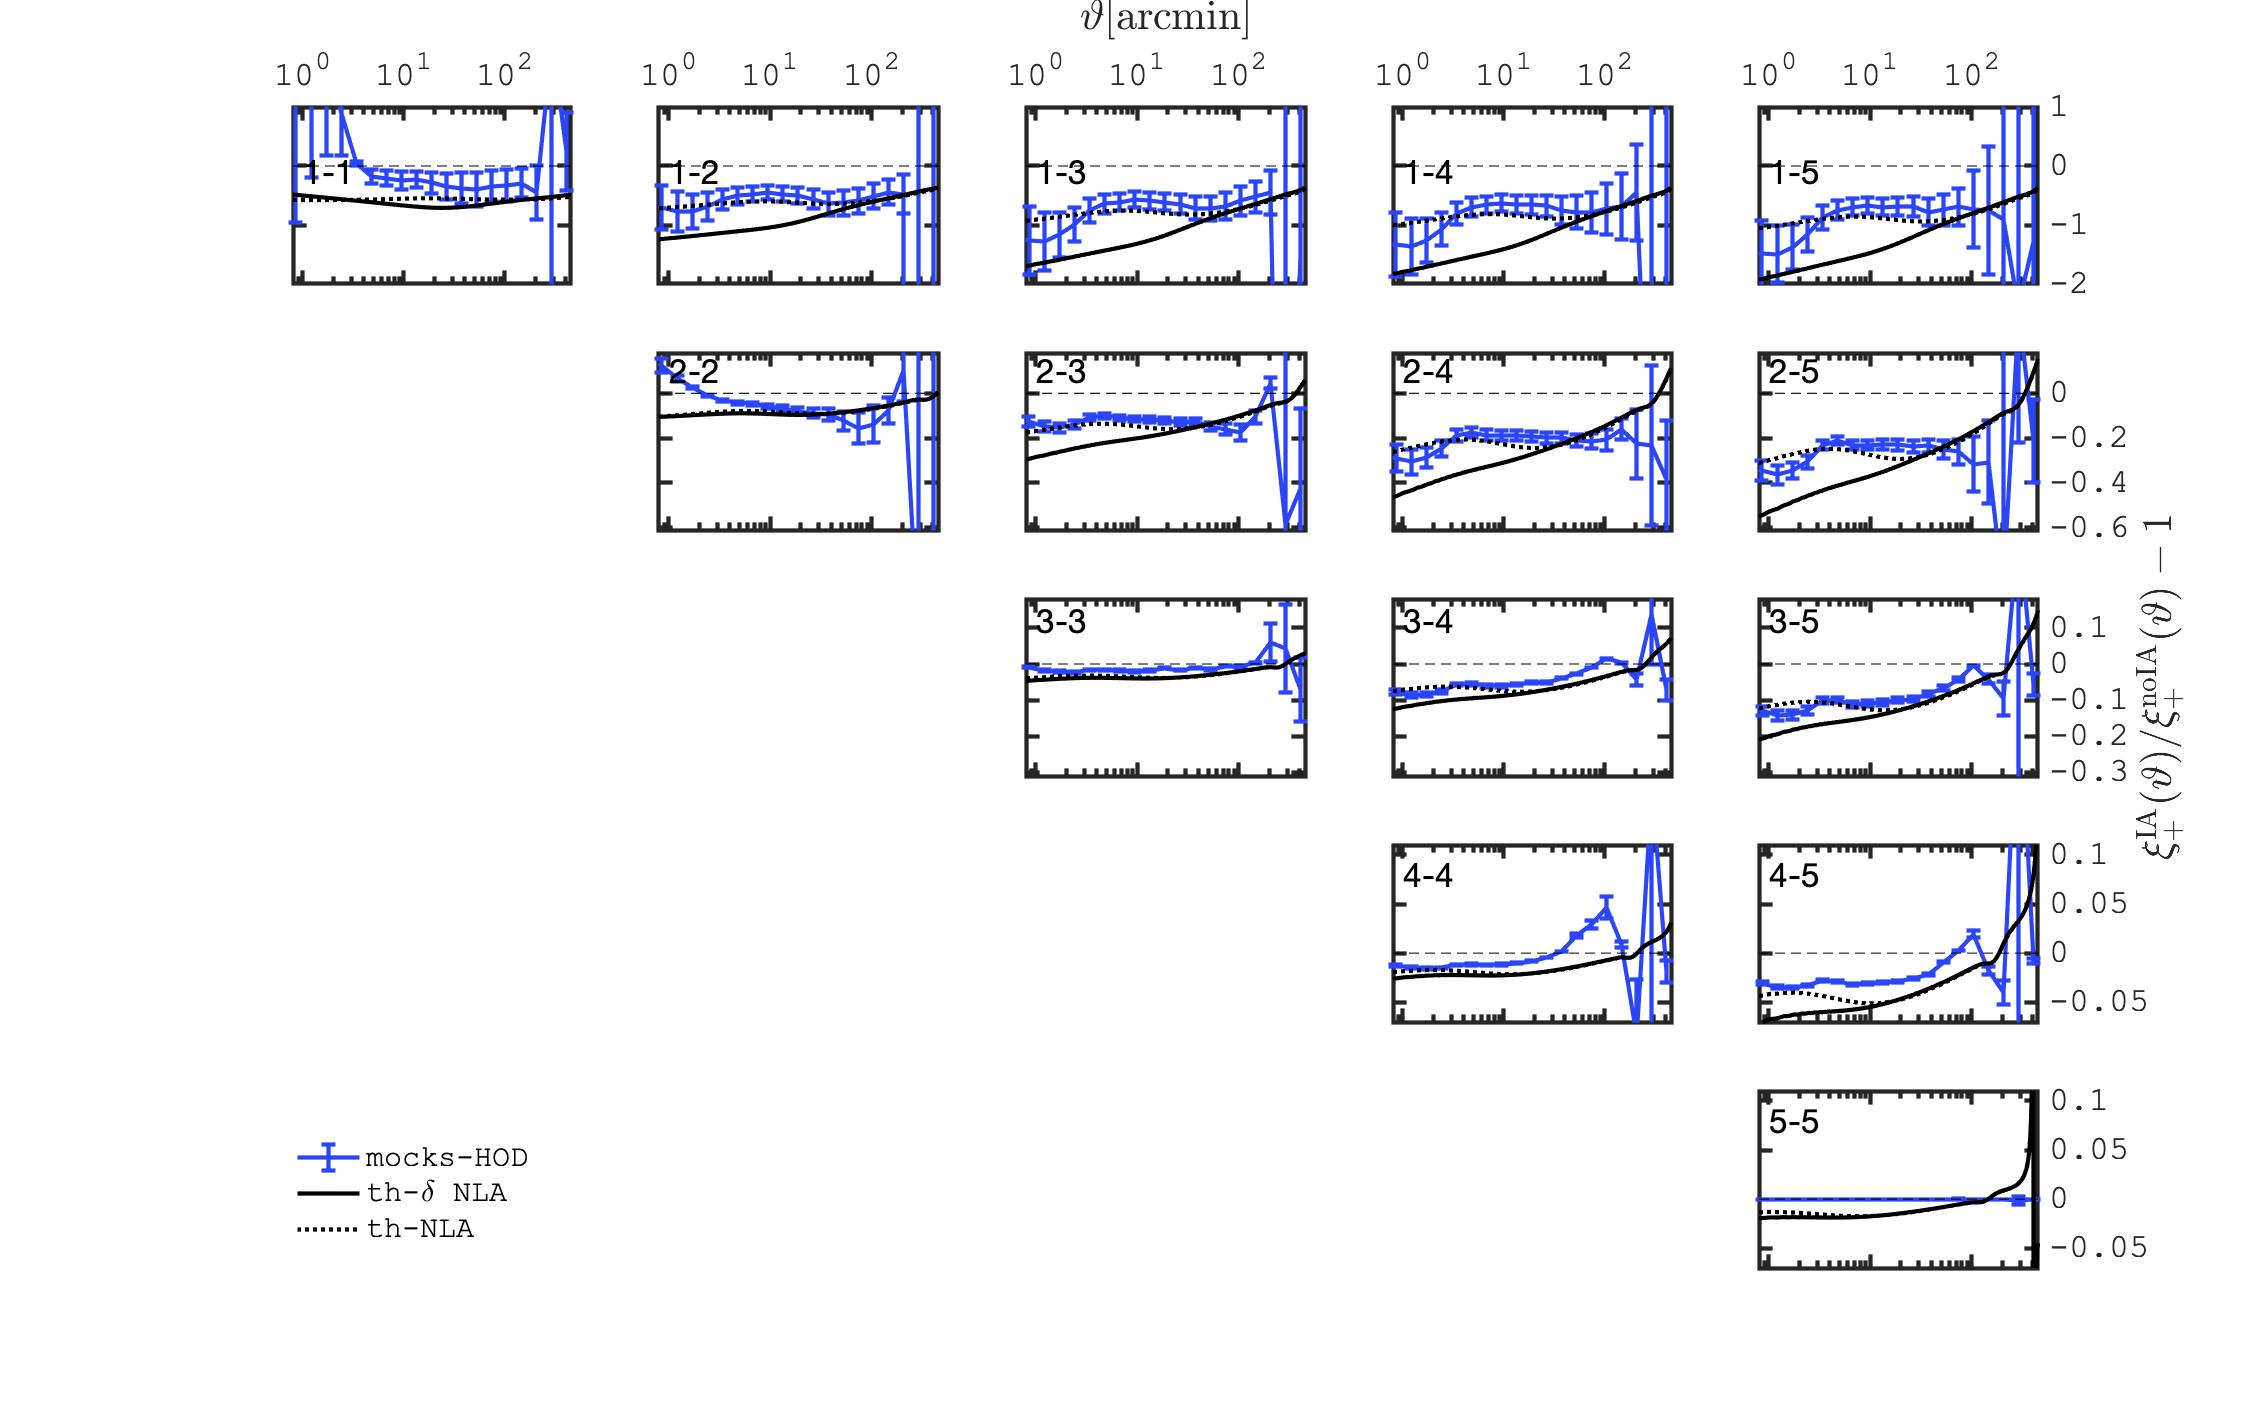
\includegraphics[width=\columnwidth]{graphs/frac_xip_sims_HOD.jpg}
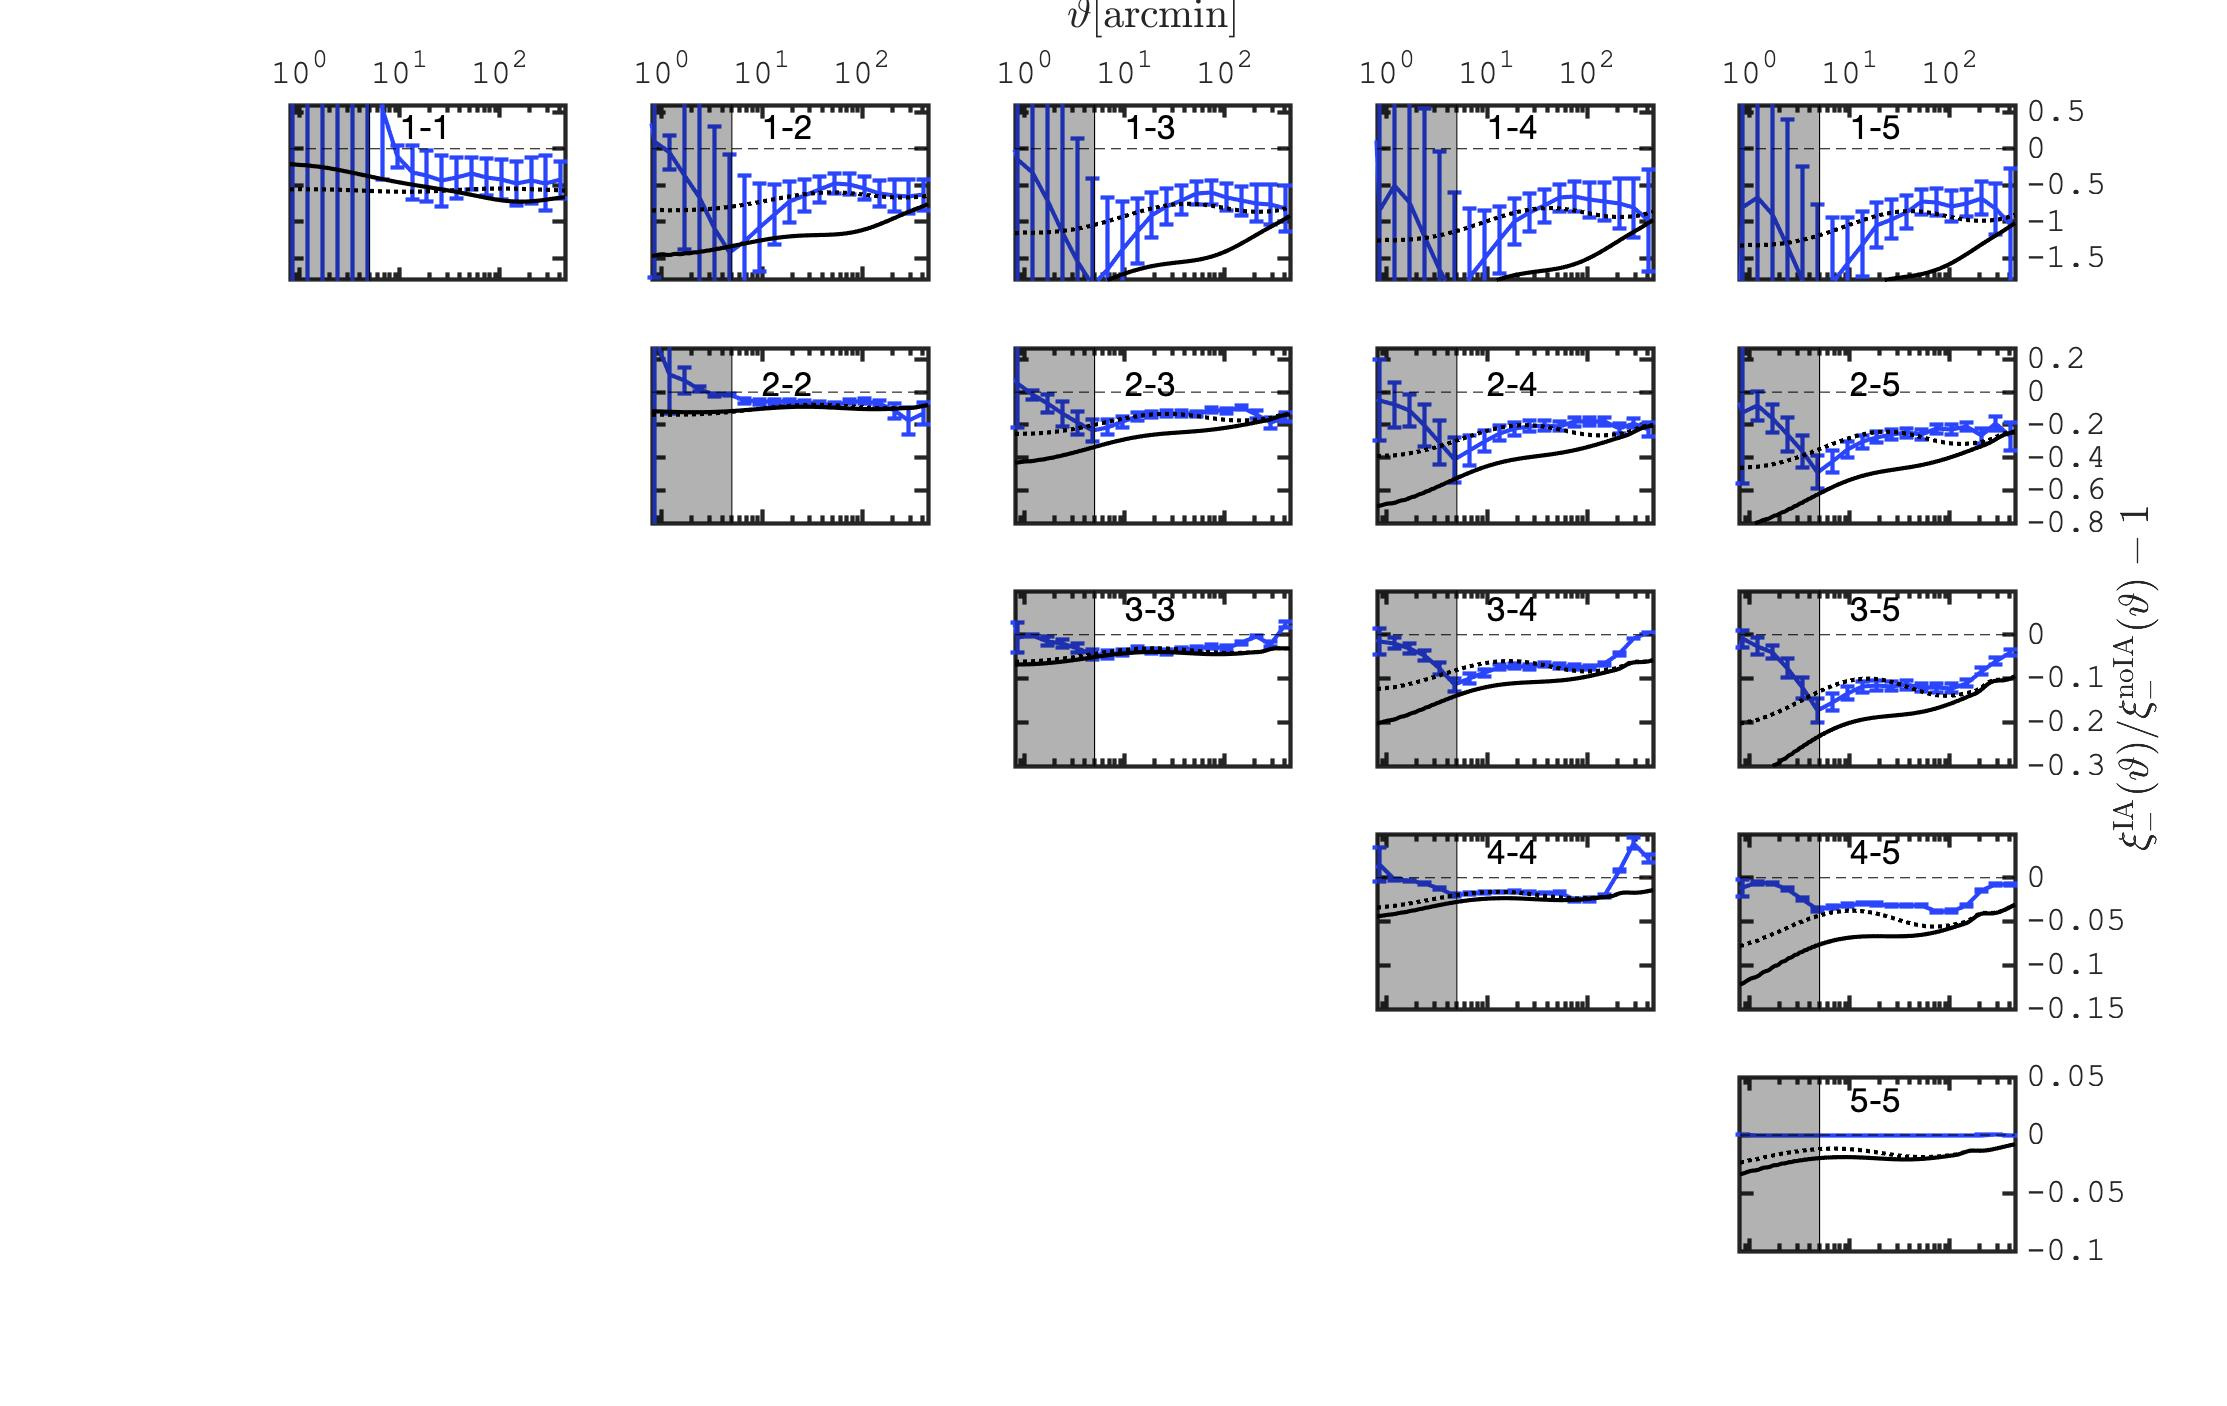
\includegraphics[width=\columnwidth]{graphs/frac_xim_sims_HOD.jpg}
\caption{Same as Fig. \ref{fig:xi_deltaNLA}, but showing the HOD galaxies with shapes linearly coupled with the tidal field. }
\label{fig:xi_hod_nla}
\end{figure*}

%--------------
\begin{figure*}
%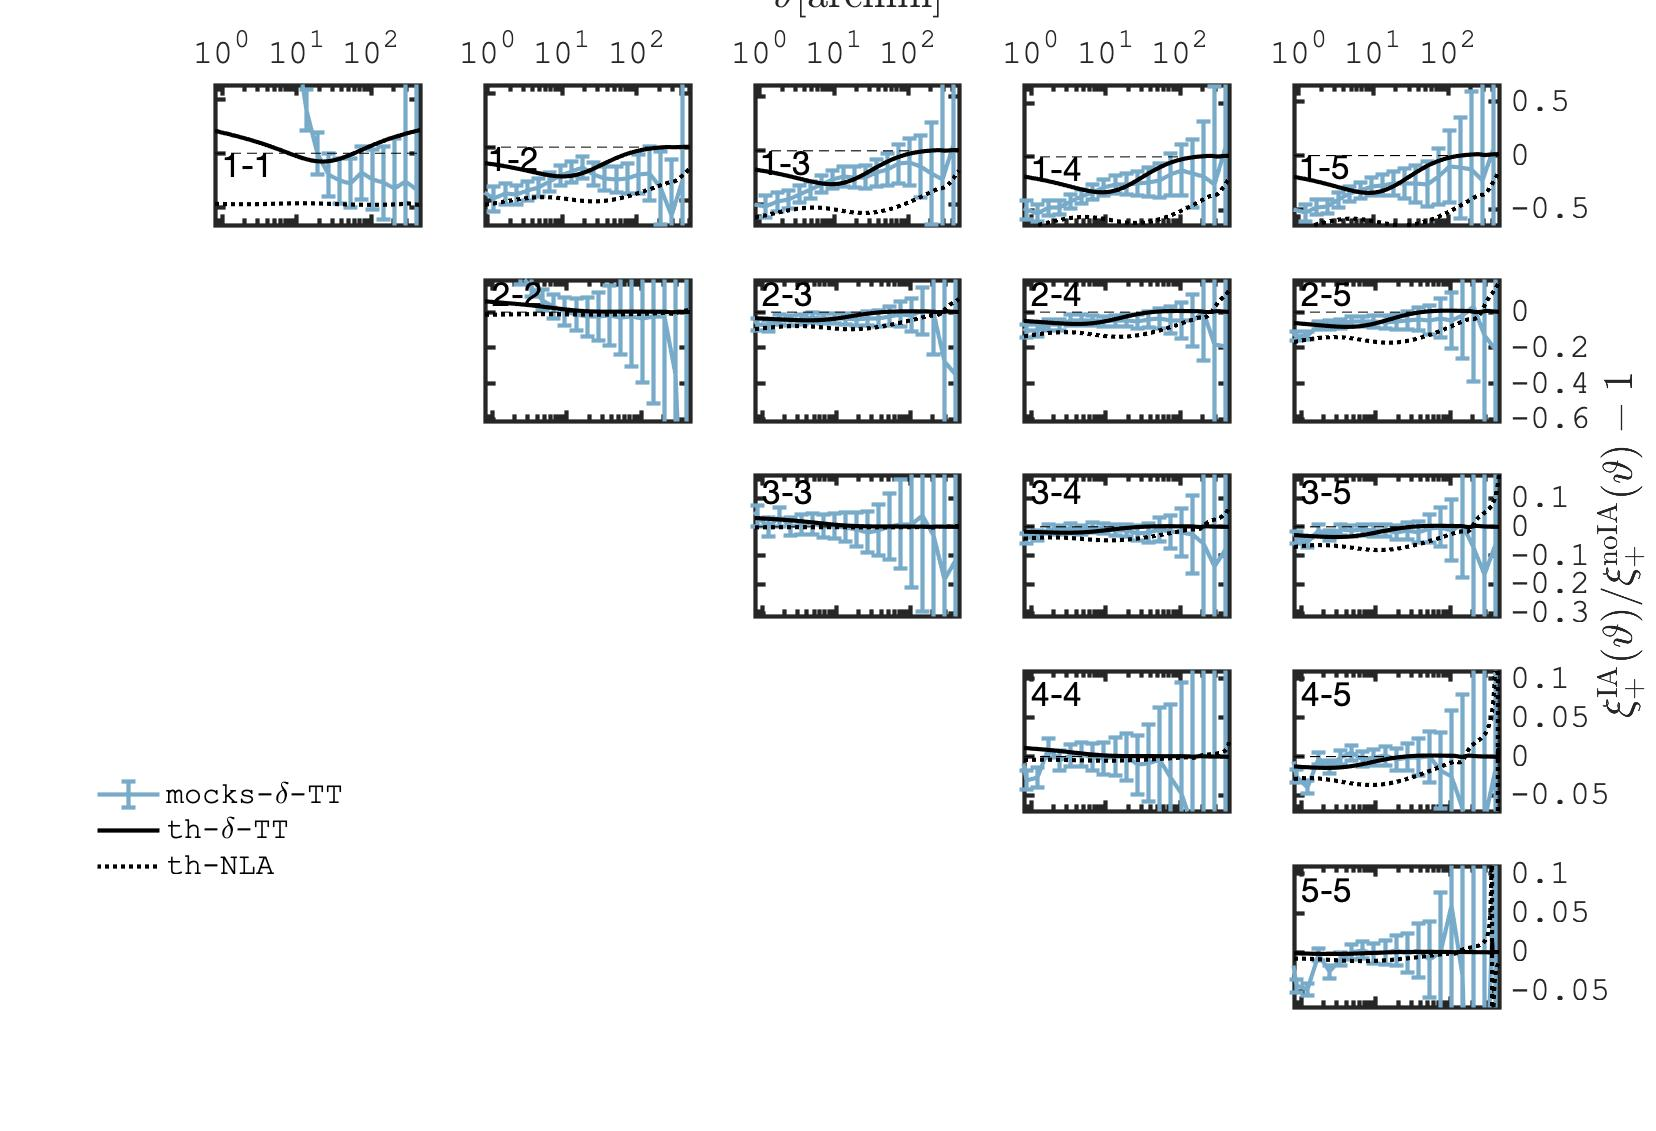
\includegraphics[width=\columnwidth]{graphs/frac_xip_C2_m1_skysim_deltaTT}
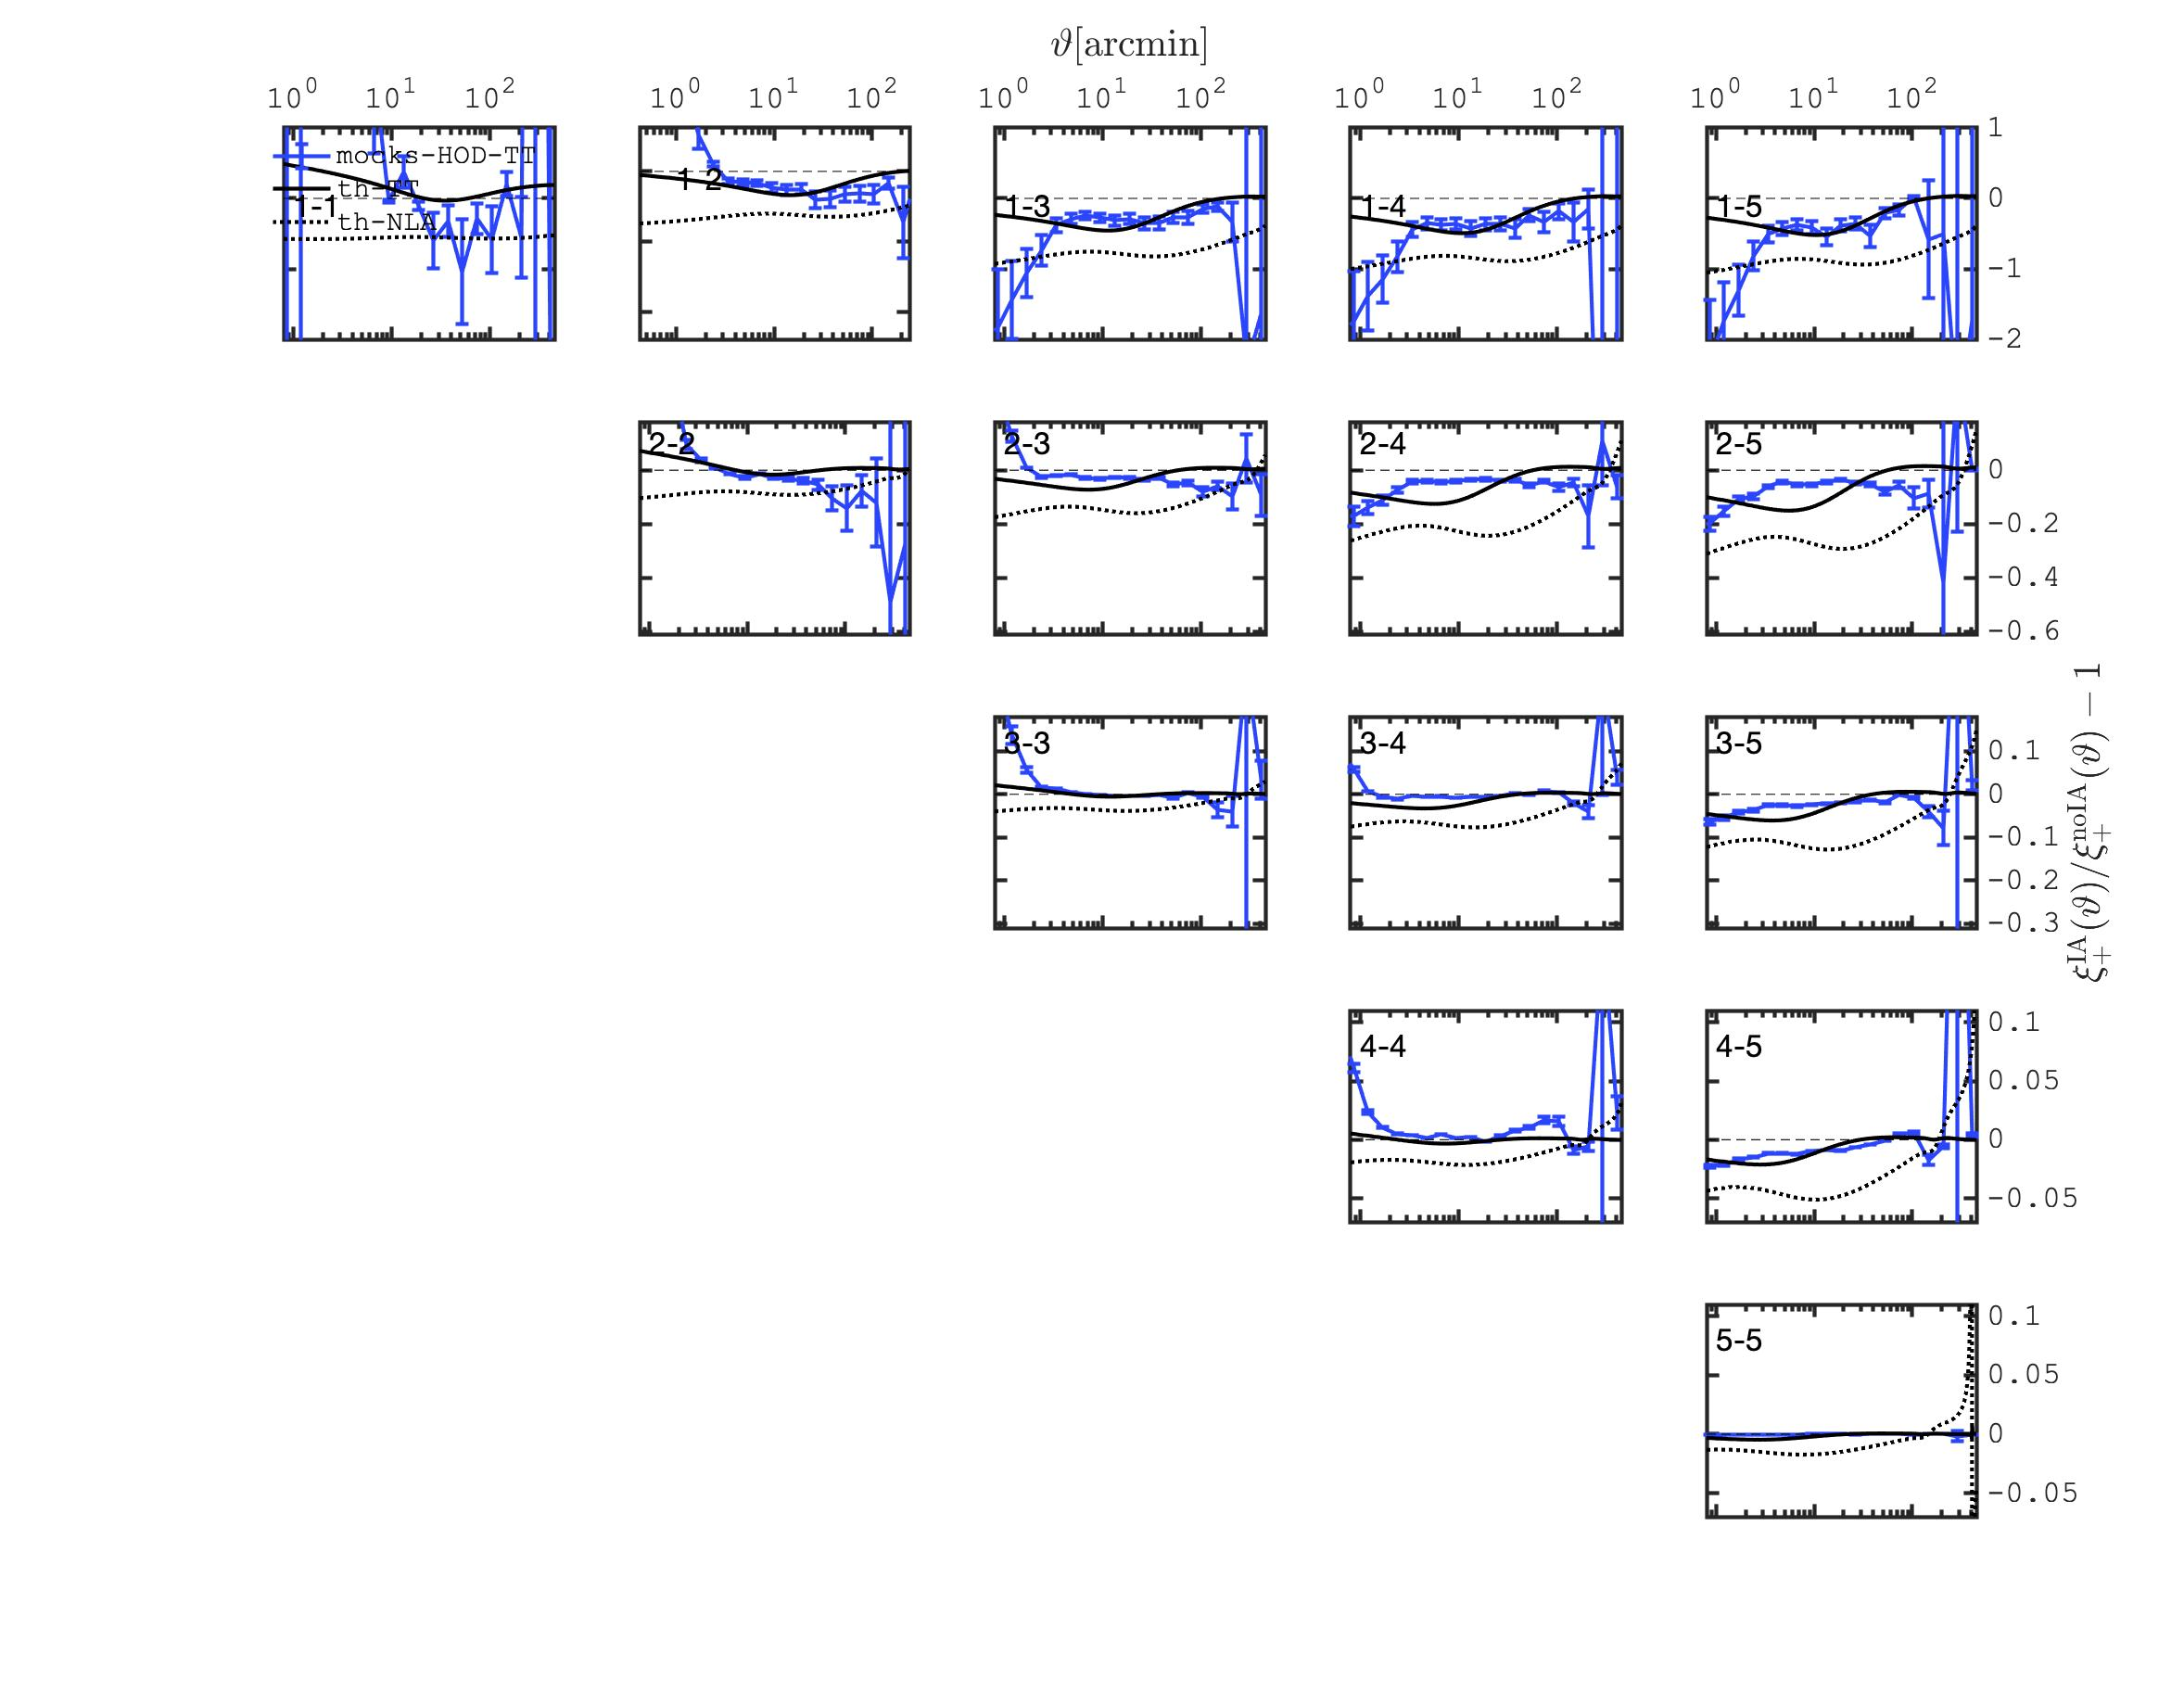
\includegraphics[width=\columnwidth]{graphs/frac_xip_sims_HOD_TT.jpg}
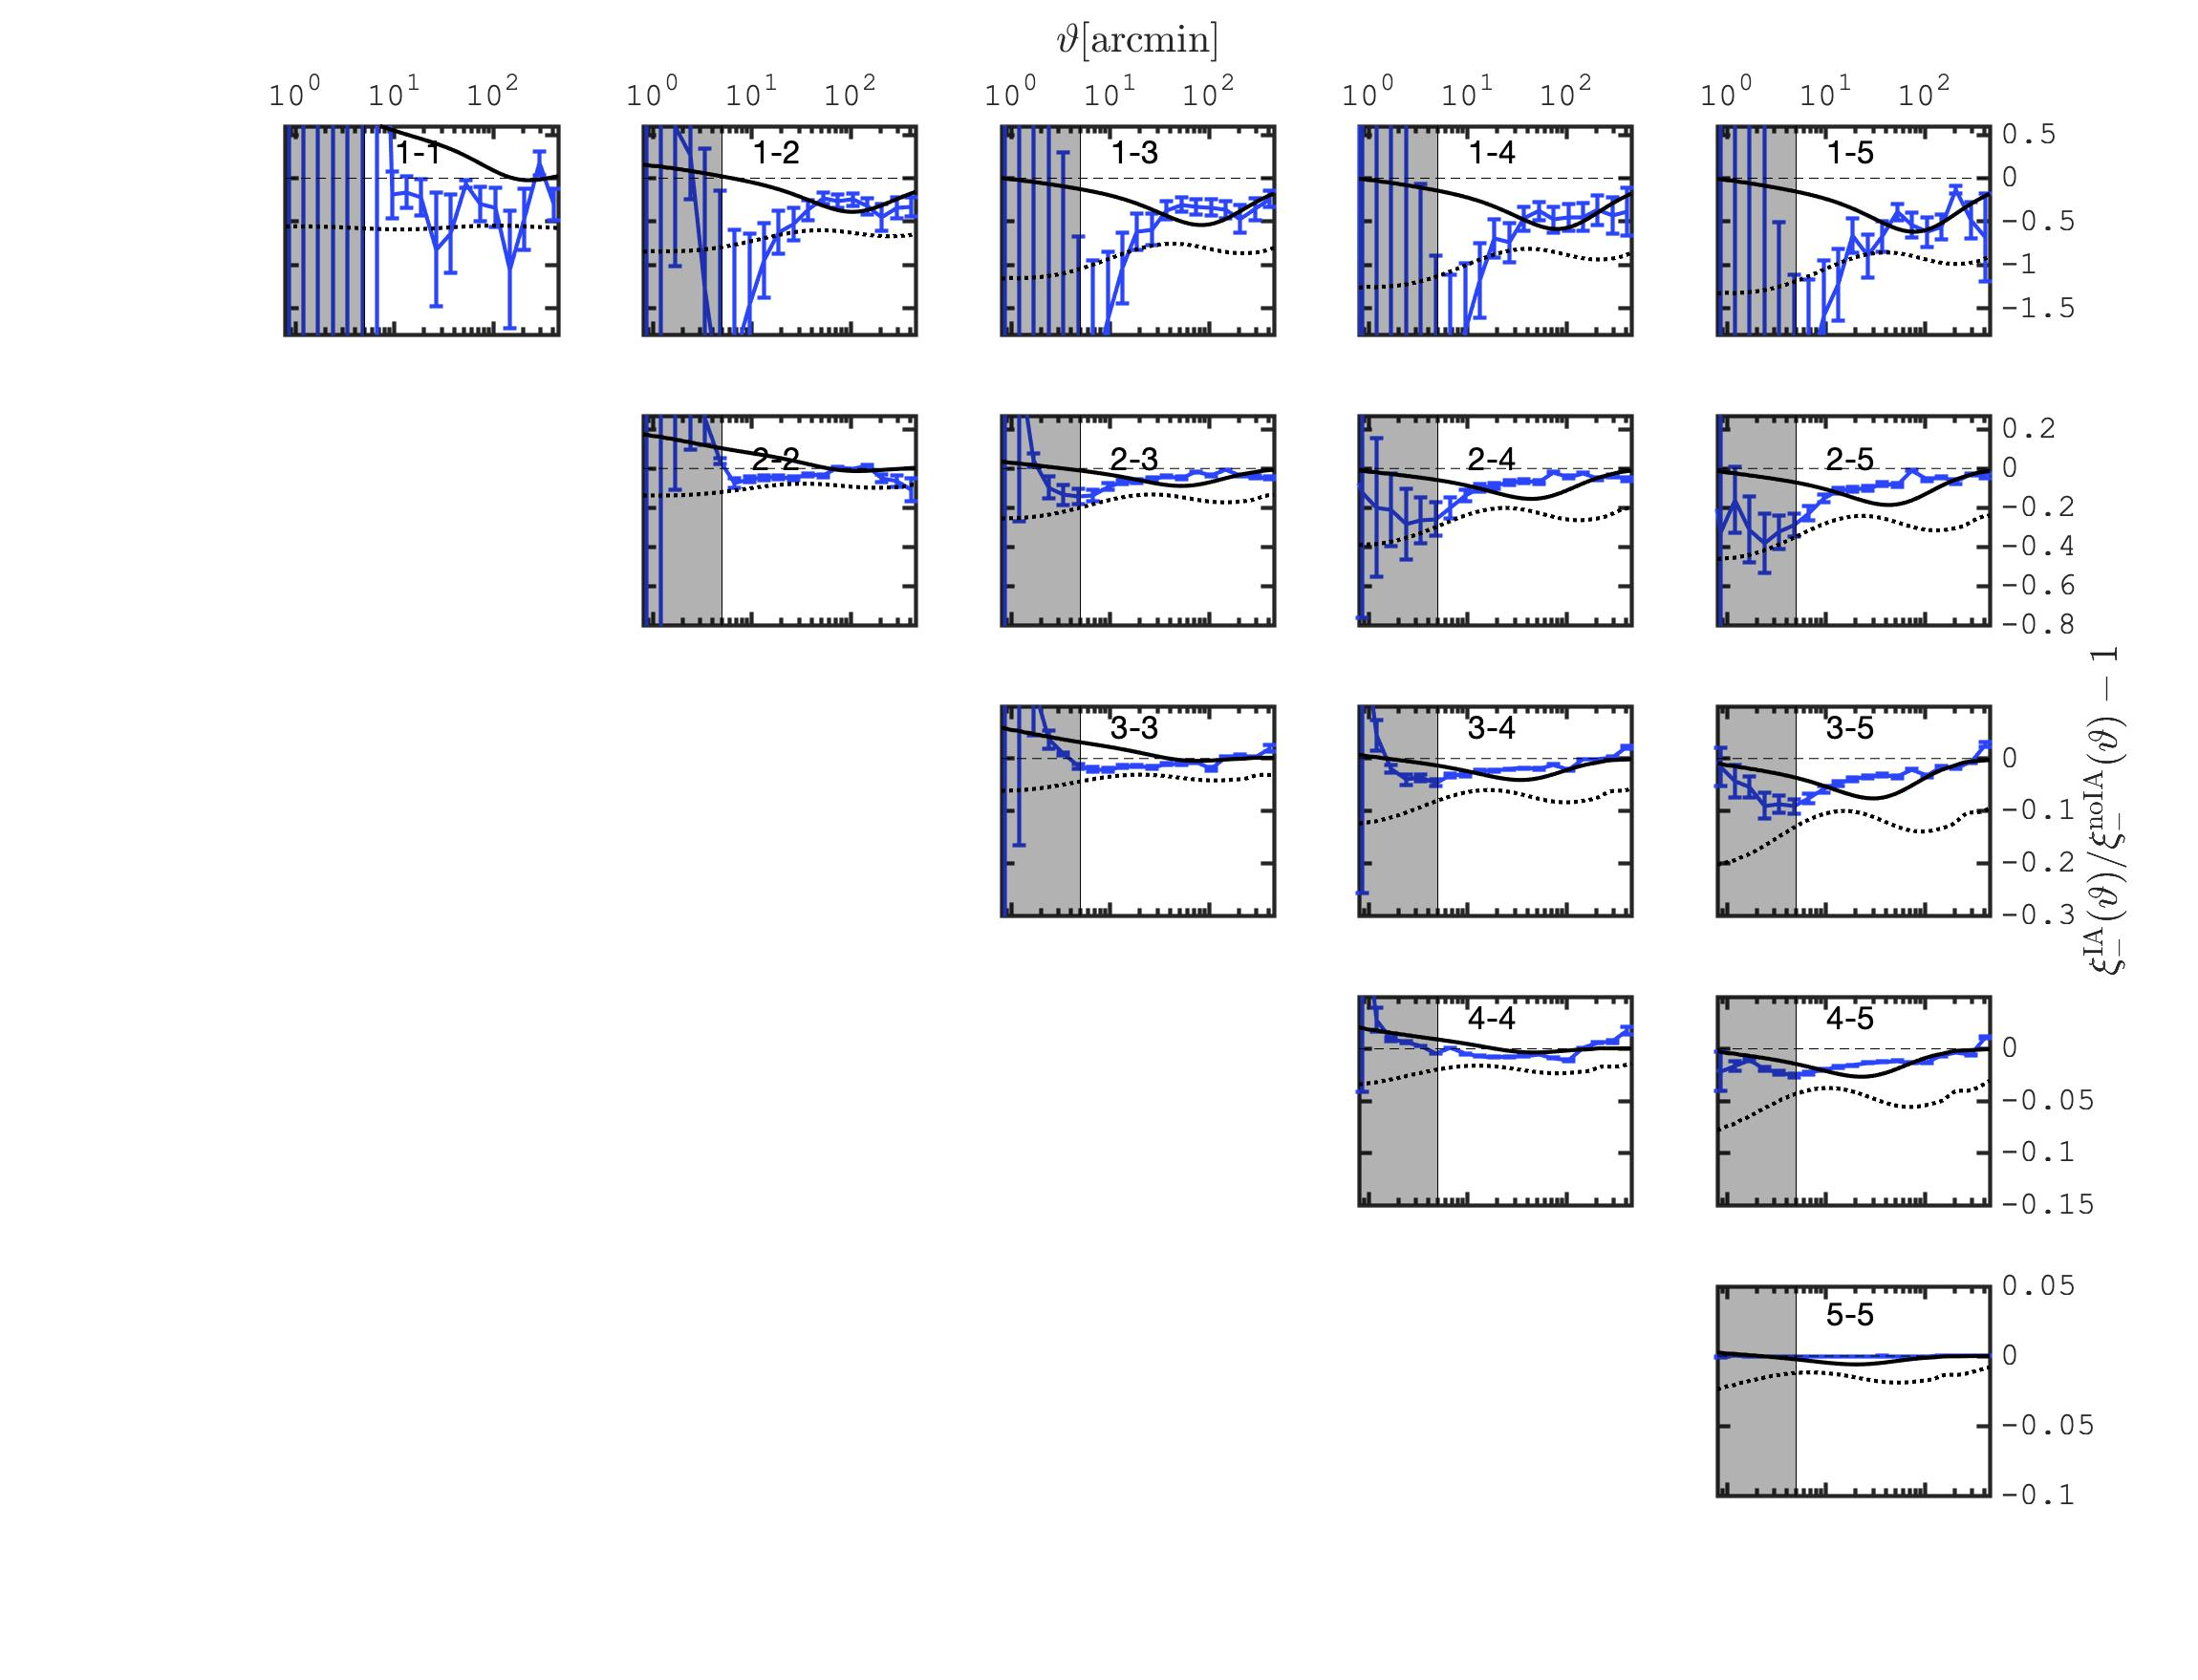
\includegraphics[width=\columnwidth]{graphs/frac_xim_sims_HOD_TT.jpg}
\caption{Same as Fig. \ref{fig:xi_deltaTT}, but showing the HOD galaxies with shapes quadratically coupled with the tidal field. }
\label{fig:xi_hod_tt}
\end{figure*}


%The NLA and extended-NLA models respectively assume a null and a linear bias between the source galaxies and the underlying matter field, both of which are approximations to the galaxy-dark matter connection.
%In fact, galaxies populate dark matter over-densities in a more complex manner \citep{GalaxyPopulationPapers}, which is better described by the Halo Occupation Distribution approach (HOD hereafter).
The largest difference between the previous models and those based on HOD galaxies is that the latter are non-linear biased tracers of the matter distribution, which means that a larger number can populate regions of large over-densities, where the tidal fields are generally stronger. We therefore expect the impact of IA to be stronger in this case. We show in Figs. \ref{fig:xi_hod_nla} and \ref{fig:xi_hod_tt} show the results from the HOD-NLA  and HOD-TT models, which together make up our HOD-TATT. One of the most interesting features is that the HOD-NLA closely follows the normal NLA predictions over a large range of scales, suggesting that the impact of the non-linear galaxy bias is sub-dominant down to a few acrmin. We also observe a small-angle up-turn in bins 1-1 and 2-2, which can be attributed to mismodelling the $II$ term (as it is the case for the extended-NLA, see the discussion above) {\it (Also what's goiing on with bin 5? There seems to be no IA signal there...)}. 



\subsection{Validation with full inference}
 \label{sec:inference}
 
 \begin{table}
   \centering
   \caption{Priors used in the likelihood sampling. {\it (verify these numbers with Niko)}}
   \tabcolsep=0.11cm
      \begin{tabular}{@{} cccccccc @{}} % Column formatting, @{} suppresses leading/trailing space
      \hline
      \hline
       Parameter       &  range & prior \\
       \hline
       Cosmology\\ 
       $\Omega_{\rm m}$ &[0.1, 0.55] & Flat\\
       $S_8$ & [0.6, 0.9] & Flat\\
       \hline
       IA\\
       $A_{\rm IA}$ & [-5, 5]&  Flat\\                    
        $b_{\rm TA}$ & [0, 2] & Flat\\
        $C_2$ & [-5, 5] & Flat\\
     \hline
    \hline 
    \end{tabular}
    \label{table:priors}
\end{table}

 
\begin{figure}
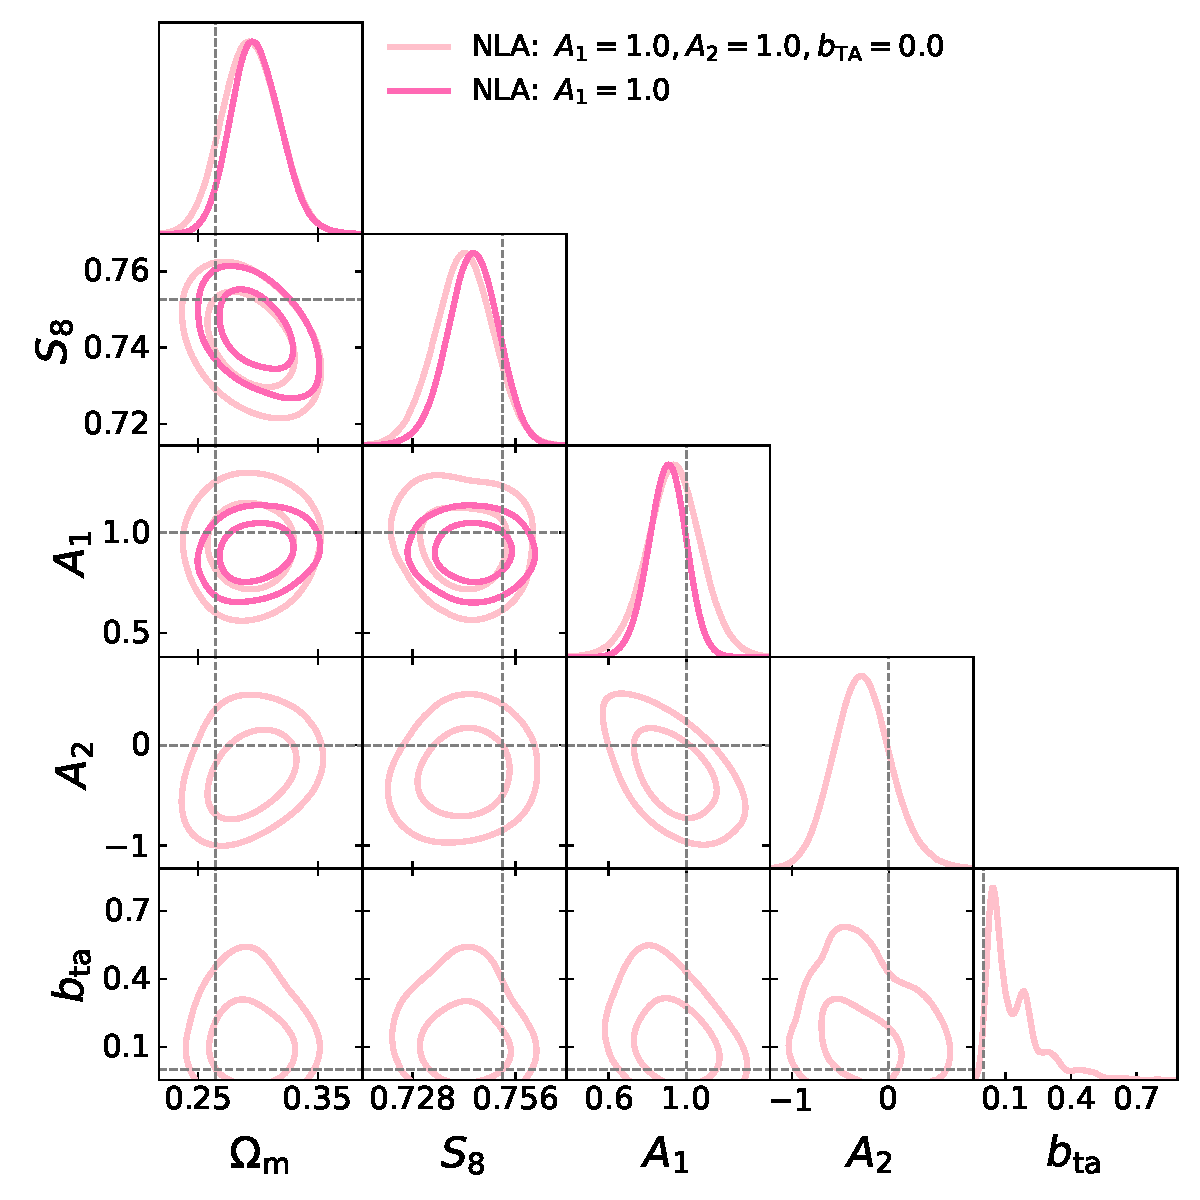
\includegraphics[width=\columnwidth]{graphs/NLA_1_0_0.pdf}
\caption{Cosmological inference from the NLA-infused simulations, with all 3 IA parameters varied (light pink) and with varying A1 only (dark pink).
The cross-hairs represent the truth as fixed in the {\it Outer Rim} $N$-body simulations \citep{OuterRim}.}
\label{fig:corner_nla_all_ia_params}
\end{figure}
\begin{figure}
%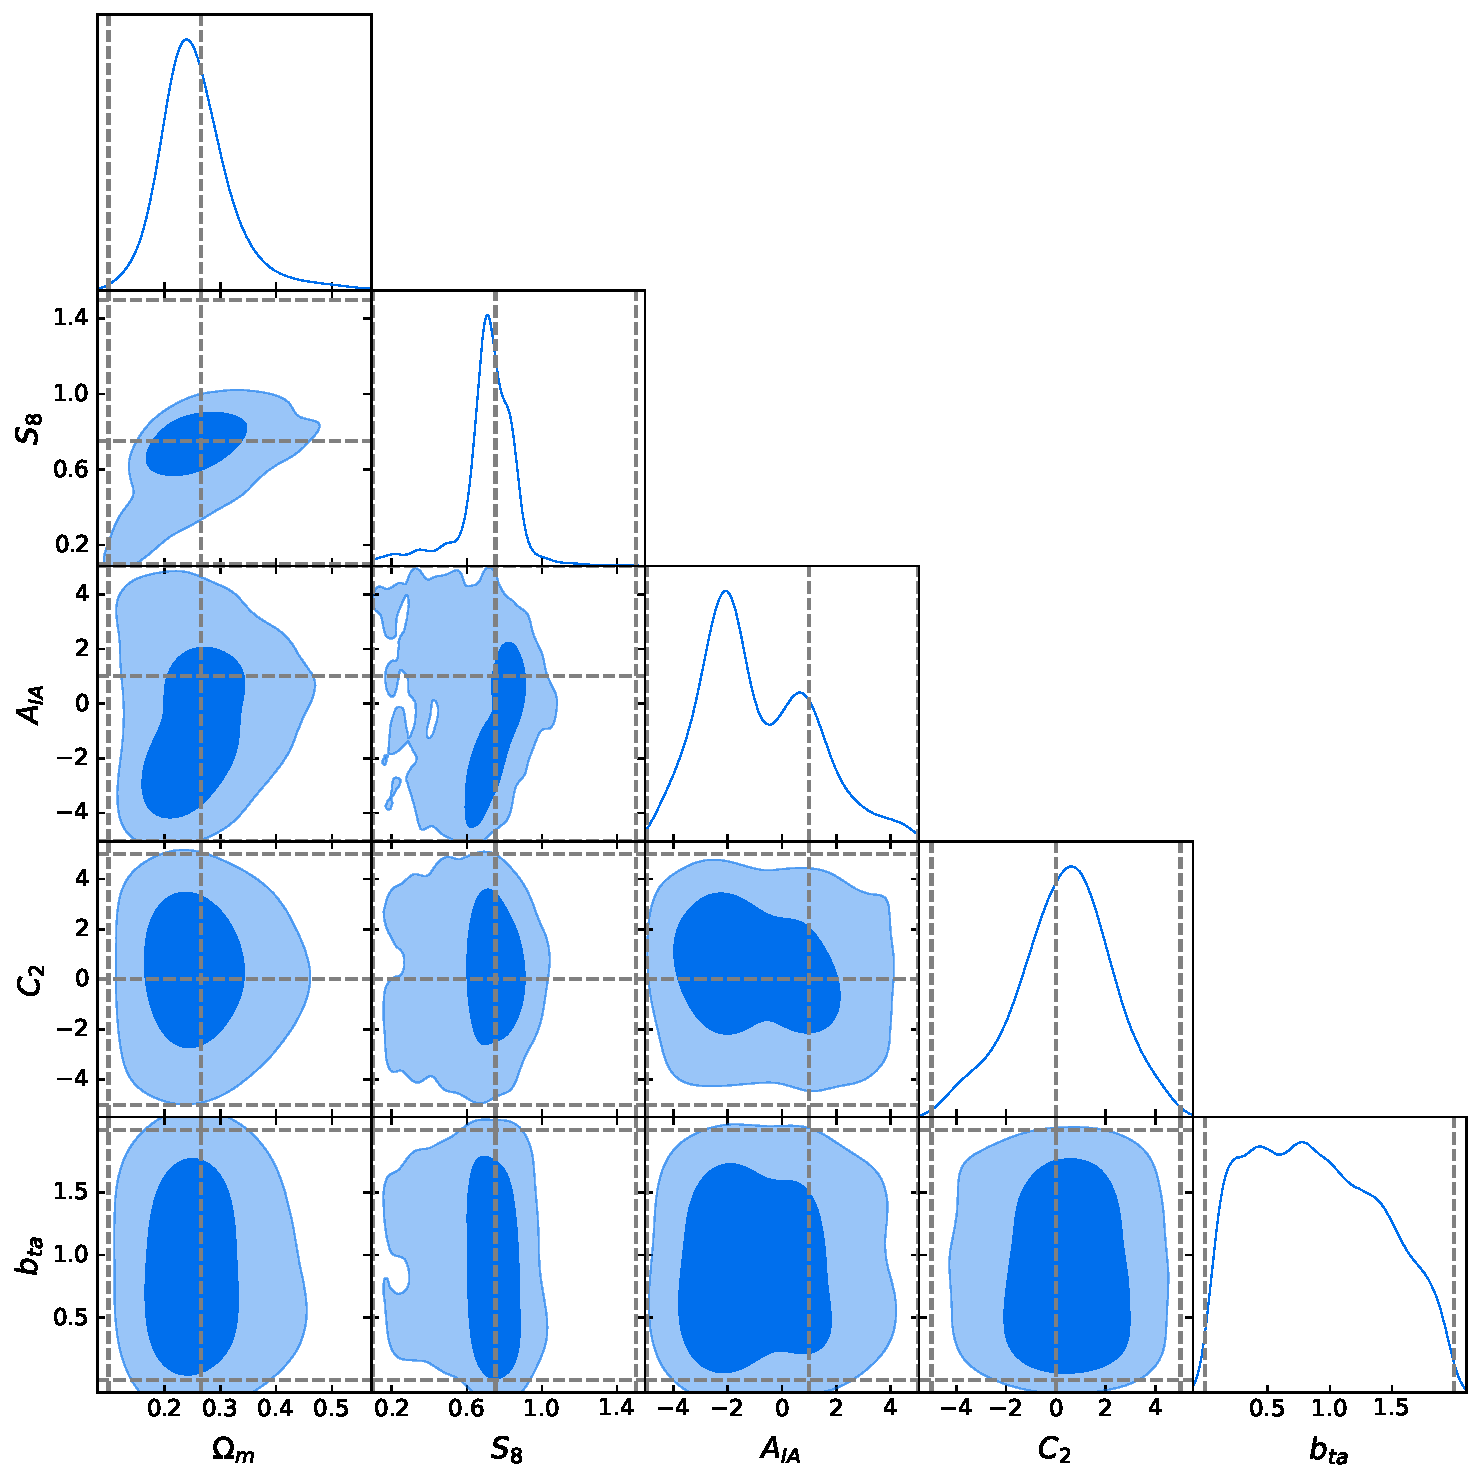
\includegraphics[width=\columnwidth]{graphs/triangle_nla_5D.pdf}
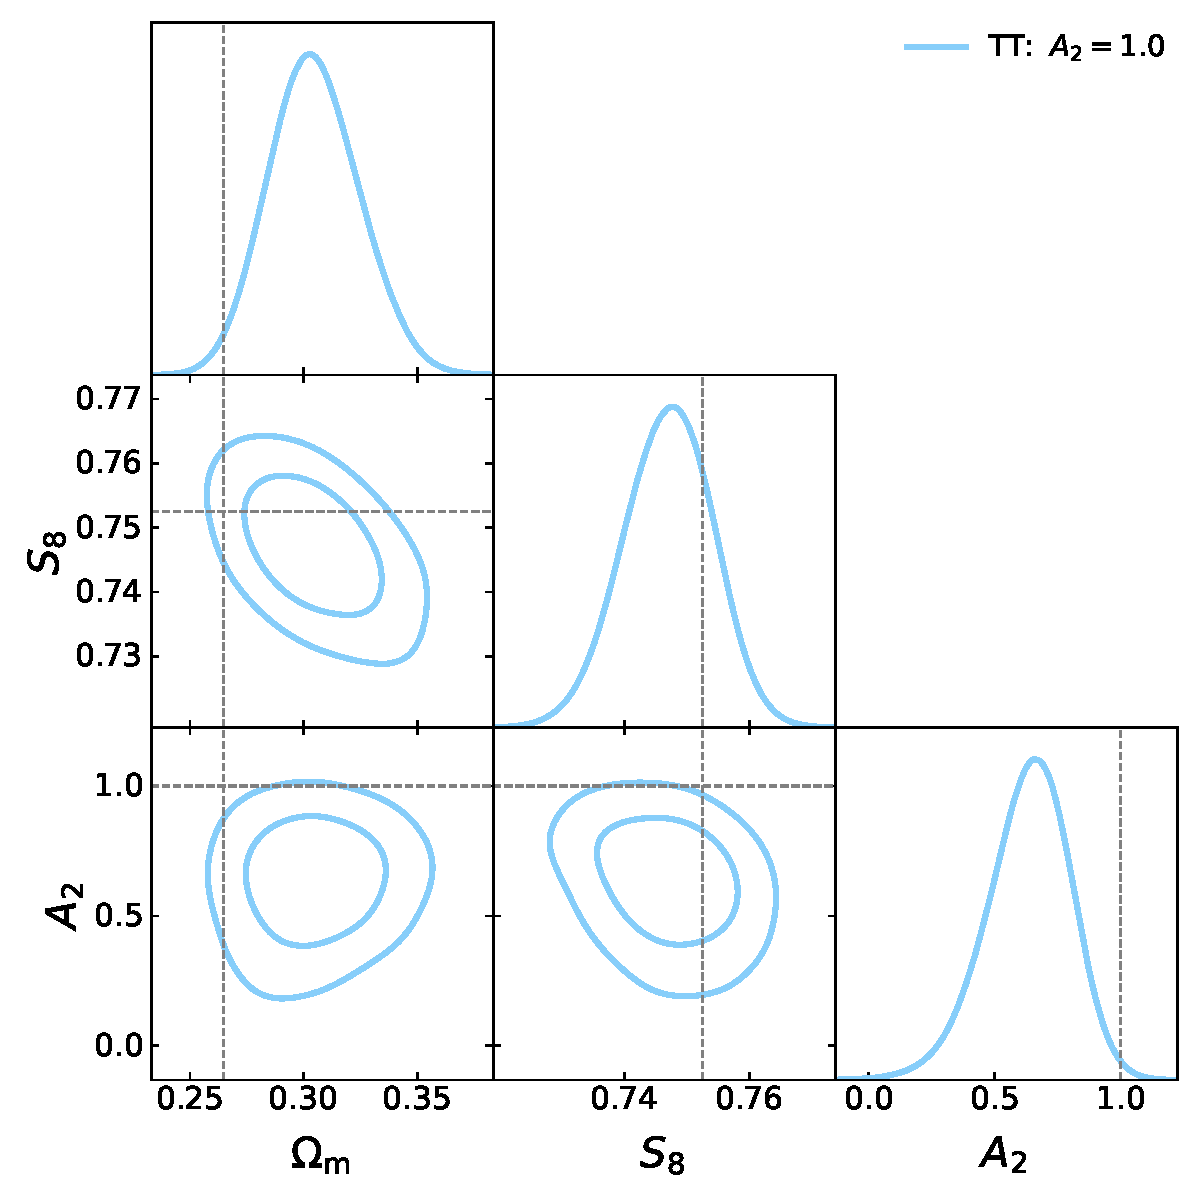
\includegraphics[width=\columnwidth]{graphs/TT_a2.pdf}
\caption{Cosmological inference from the TT-infused simulations, with $A_2$ varied ($A_1$ and $b_\mathrm{TA}$ fixed). The cross-hairs represent the truth as fixed in the {\it Outer Rim} $N$-body simulations \citep{OuterRim}.}
\label{fig:triangle_tt_vary_a2}
\end{figure}
\begin{figure}
%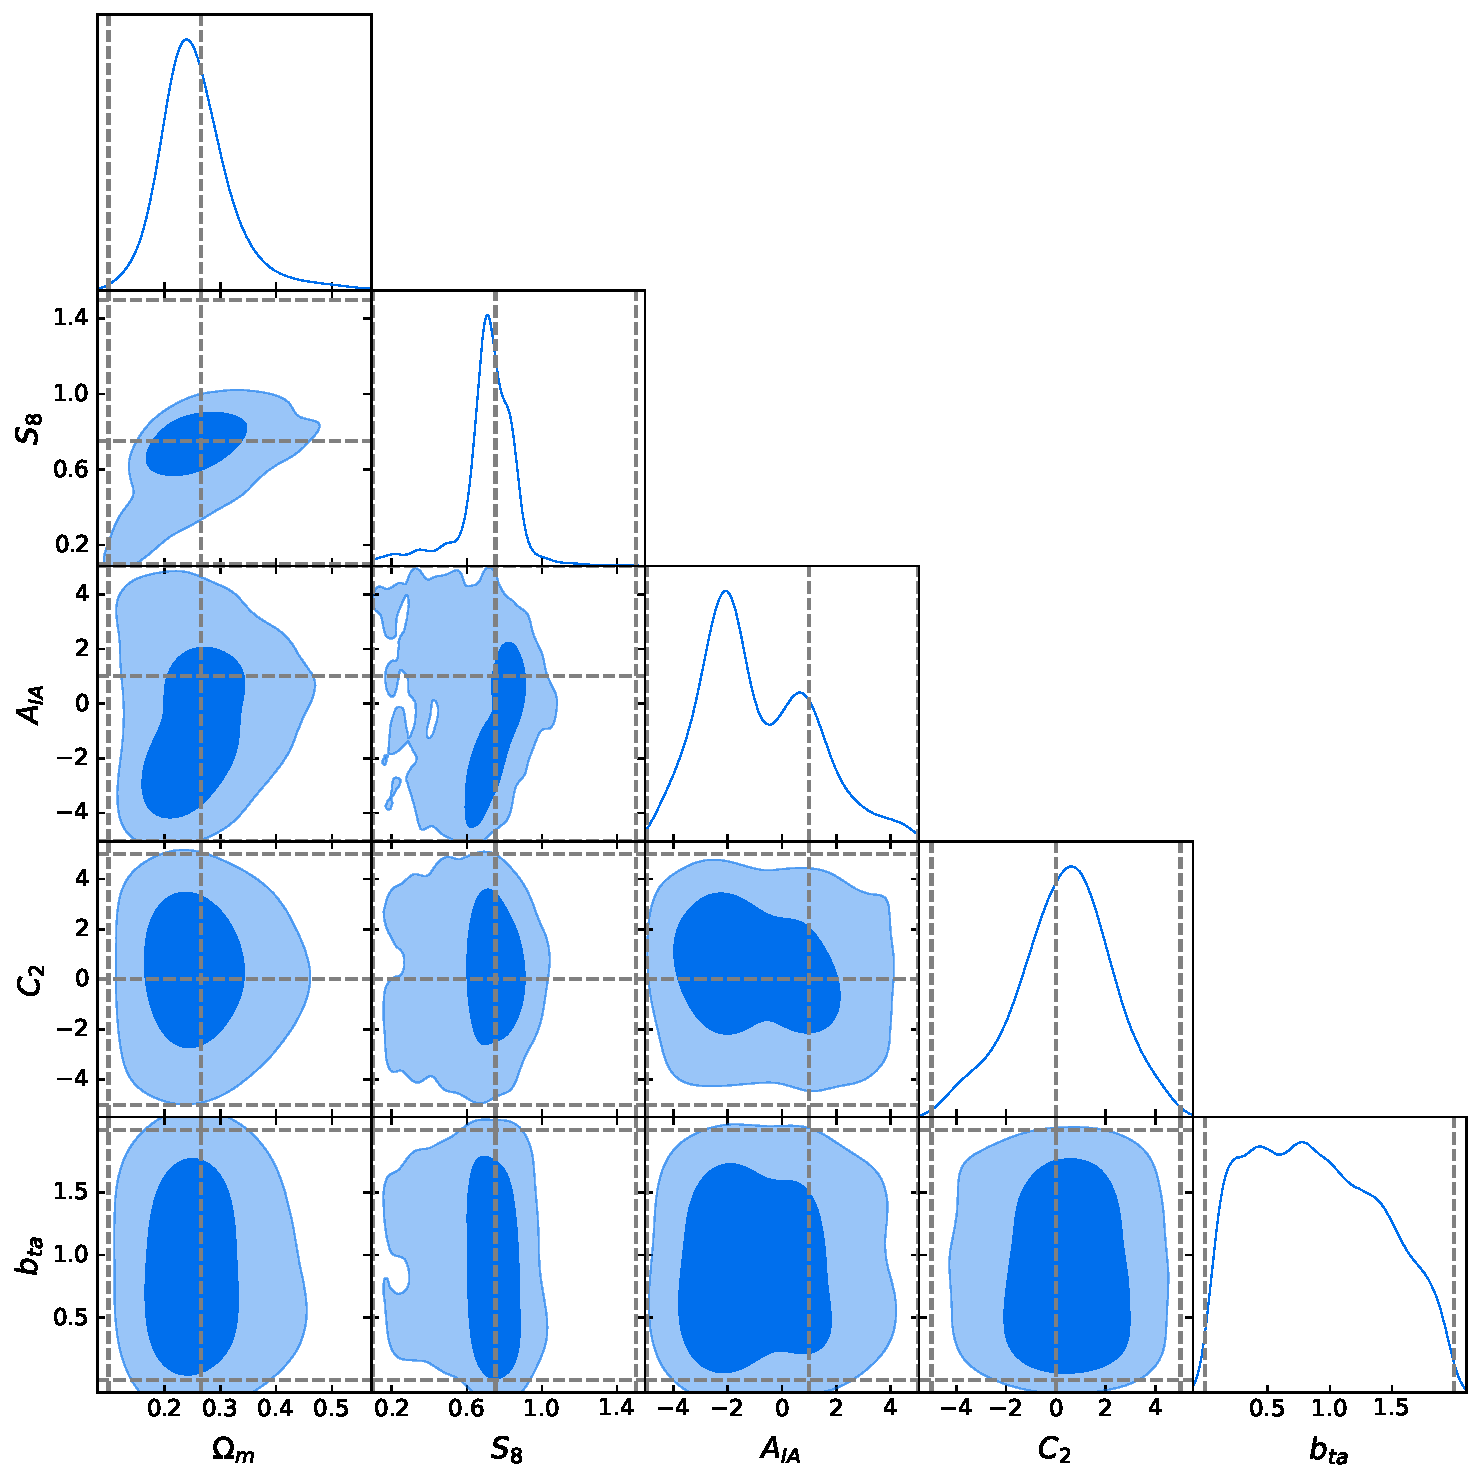
\includegraphics[width=\columnwidth]{graphs/triangle_nla_5D.pdf}
%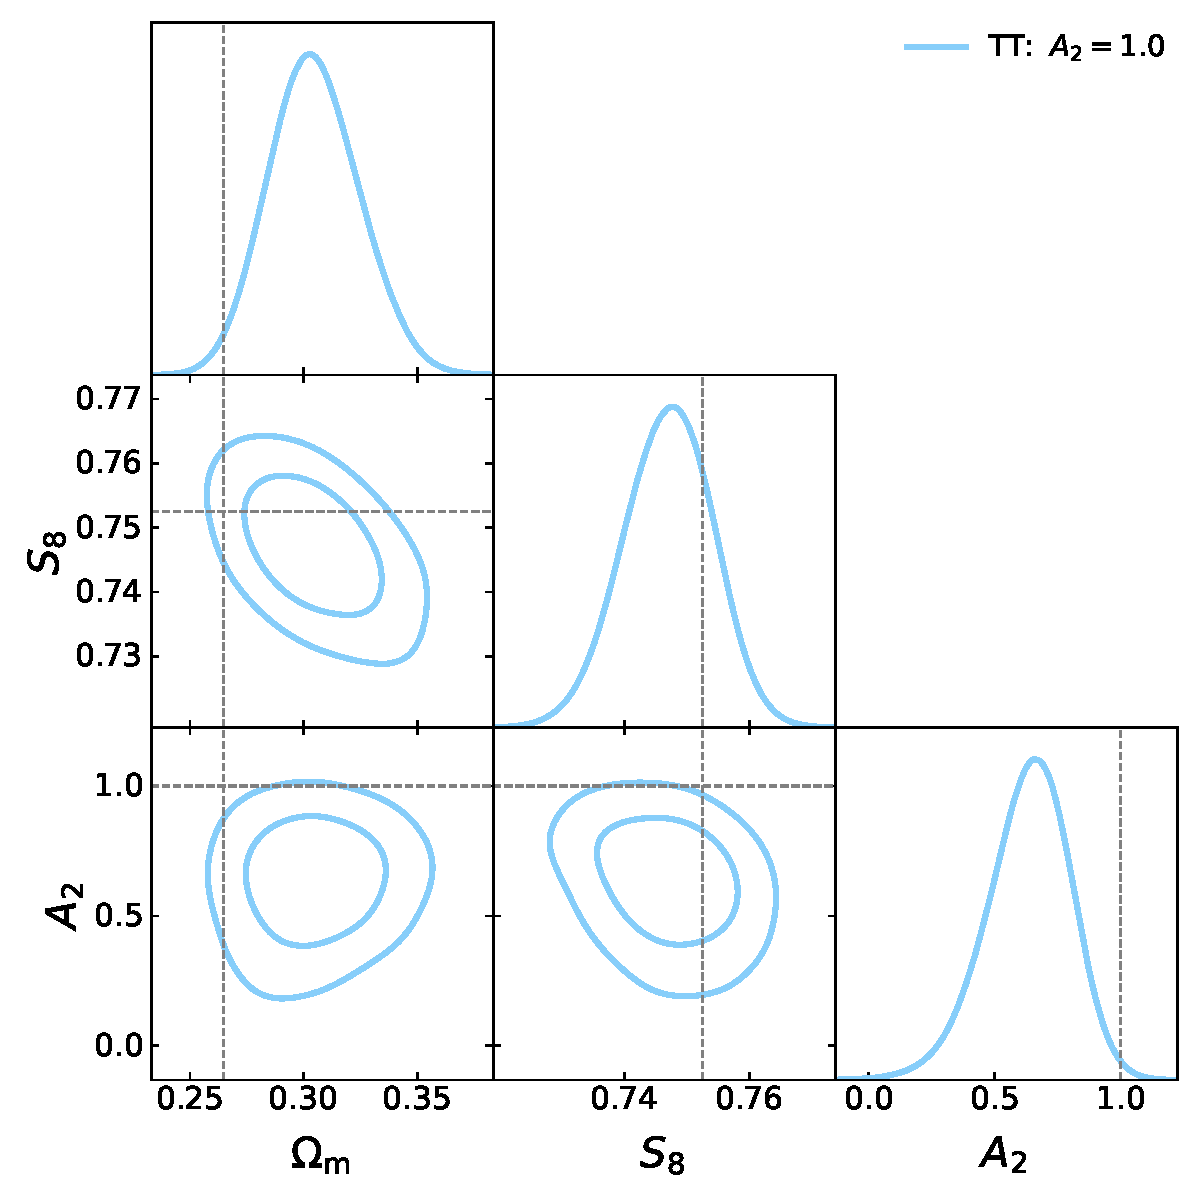
\includegraphics[width=\columnwidth]{graphs/TT_a2.pdf}
\includegraphics[width=\columnwidth]{graphs/delta_NLA.pdf}
\caption{Cosmological inference from the extended NLA-infused simulations, where either all three TATT parameters are varied.  {\it(fix axis labels and legend, remove one of the curves.)}}
\label{fig:triangle_deltaNLA_combo}
\end{figure}
\begin{figure}
%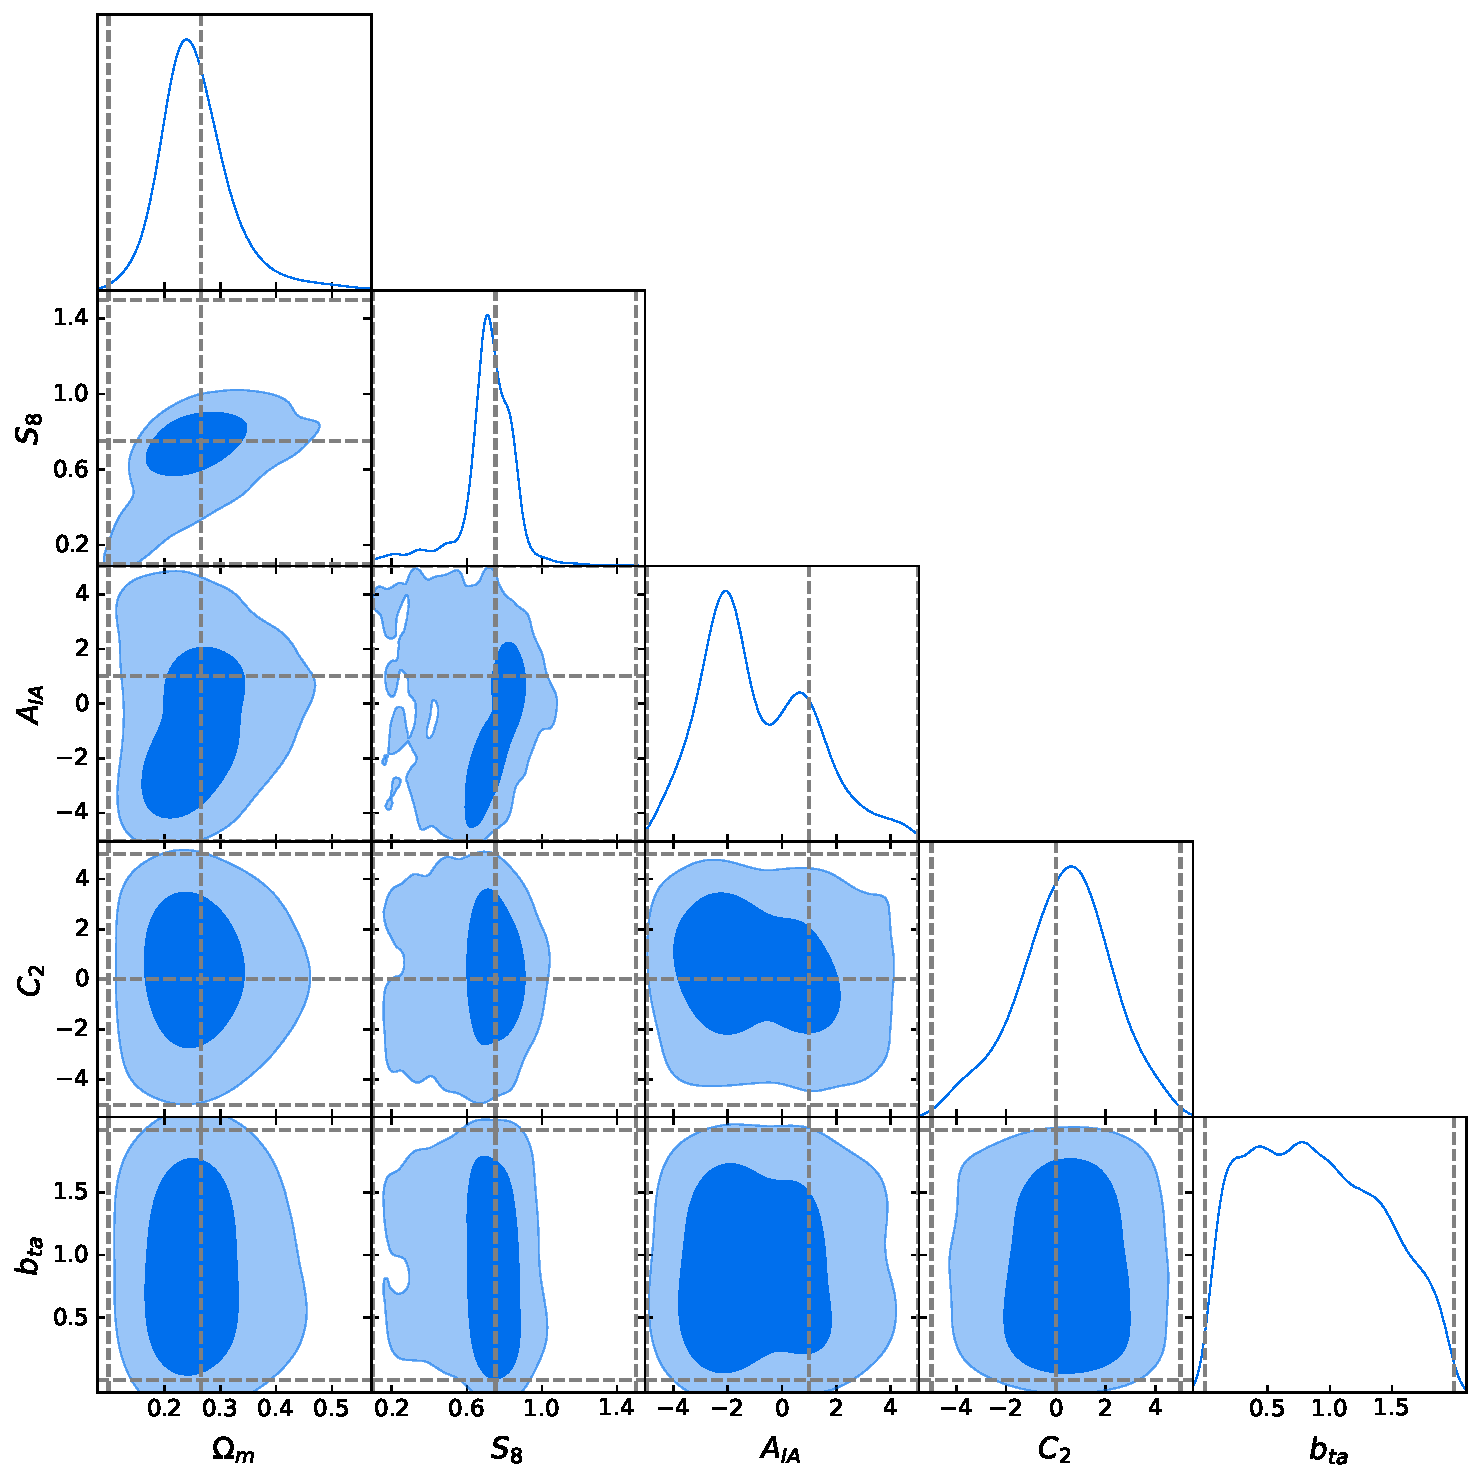
\includegraphics[width=\columnwidth]{graphs/triangle_nla_5D.pdf}
%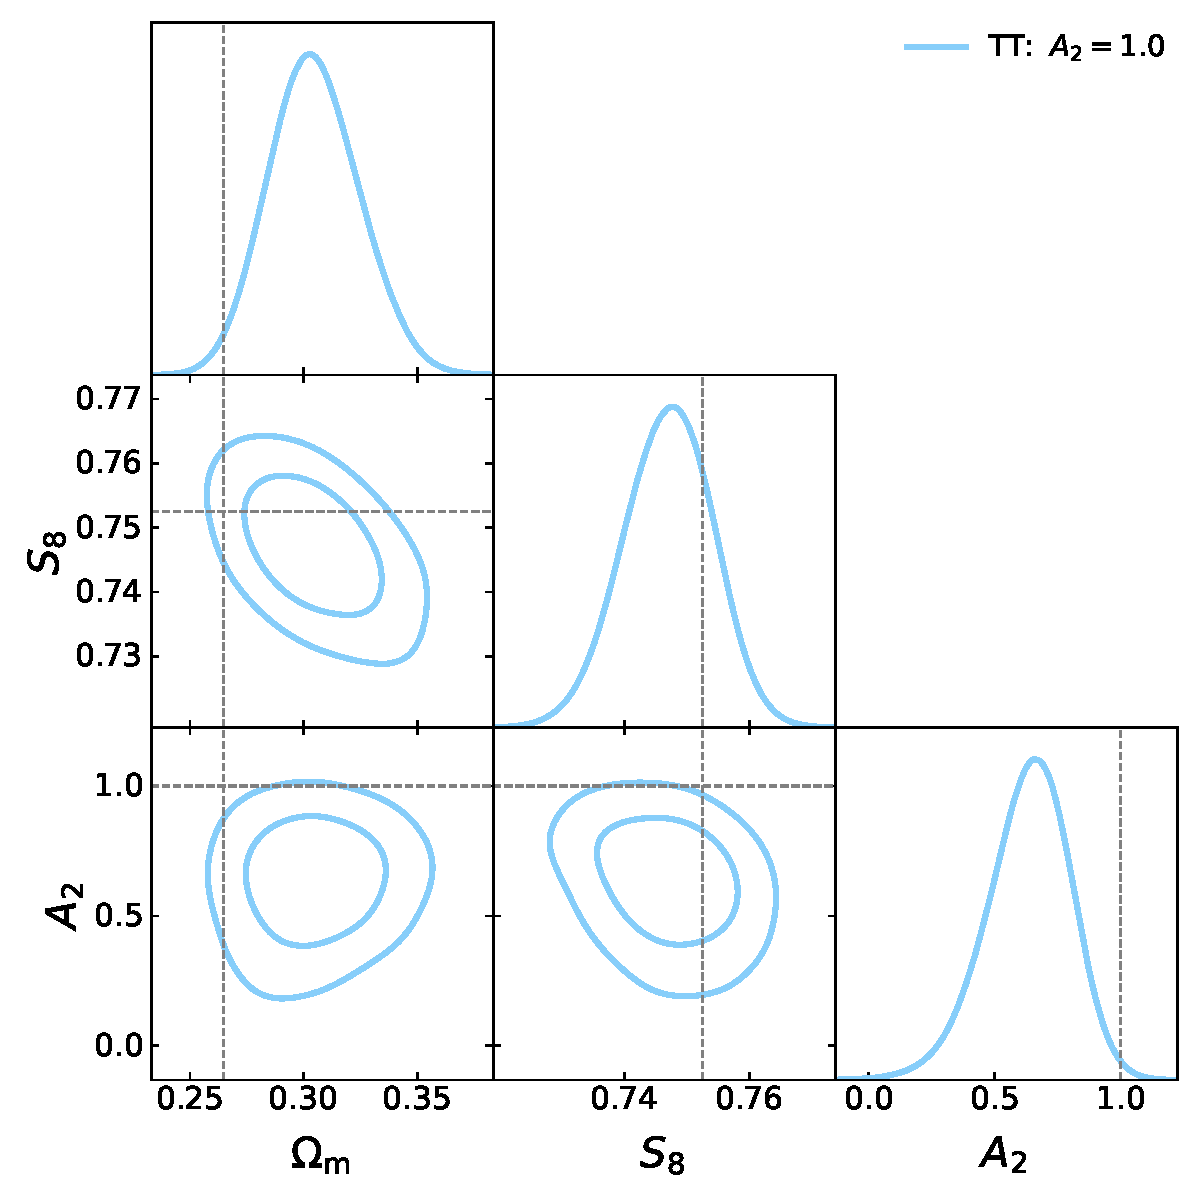
\includegraphics[width=\columnwidth]{graphs/TT_a2.pdf}
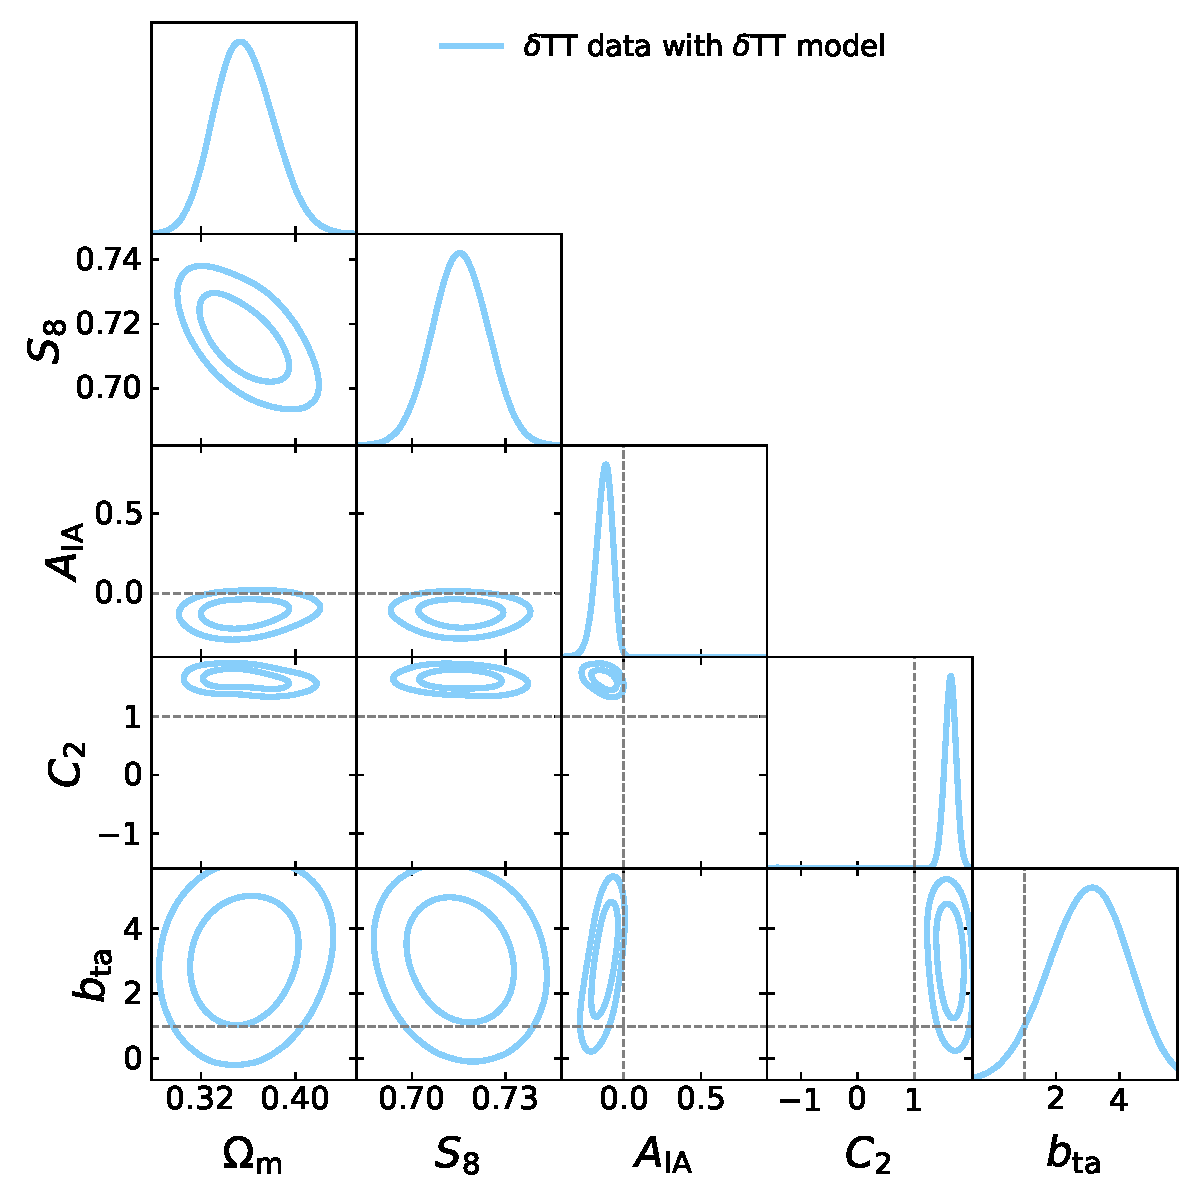
\includegraphics[width=\columnwidth]{graphs/deltaTT.pdf}
\caption{Cosmological inference from the $\delta$-TT-infused simulations, where either all three TATT parameters are varied.}
\label{fig:corner_deltatt}
\end{figure}
\begin{figure}
%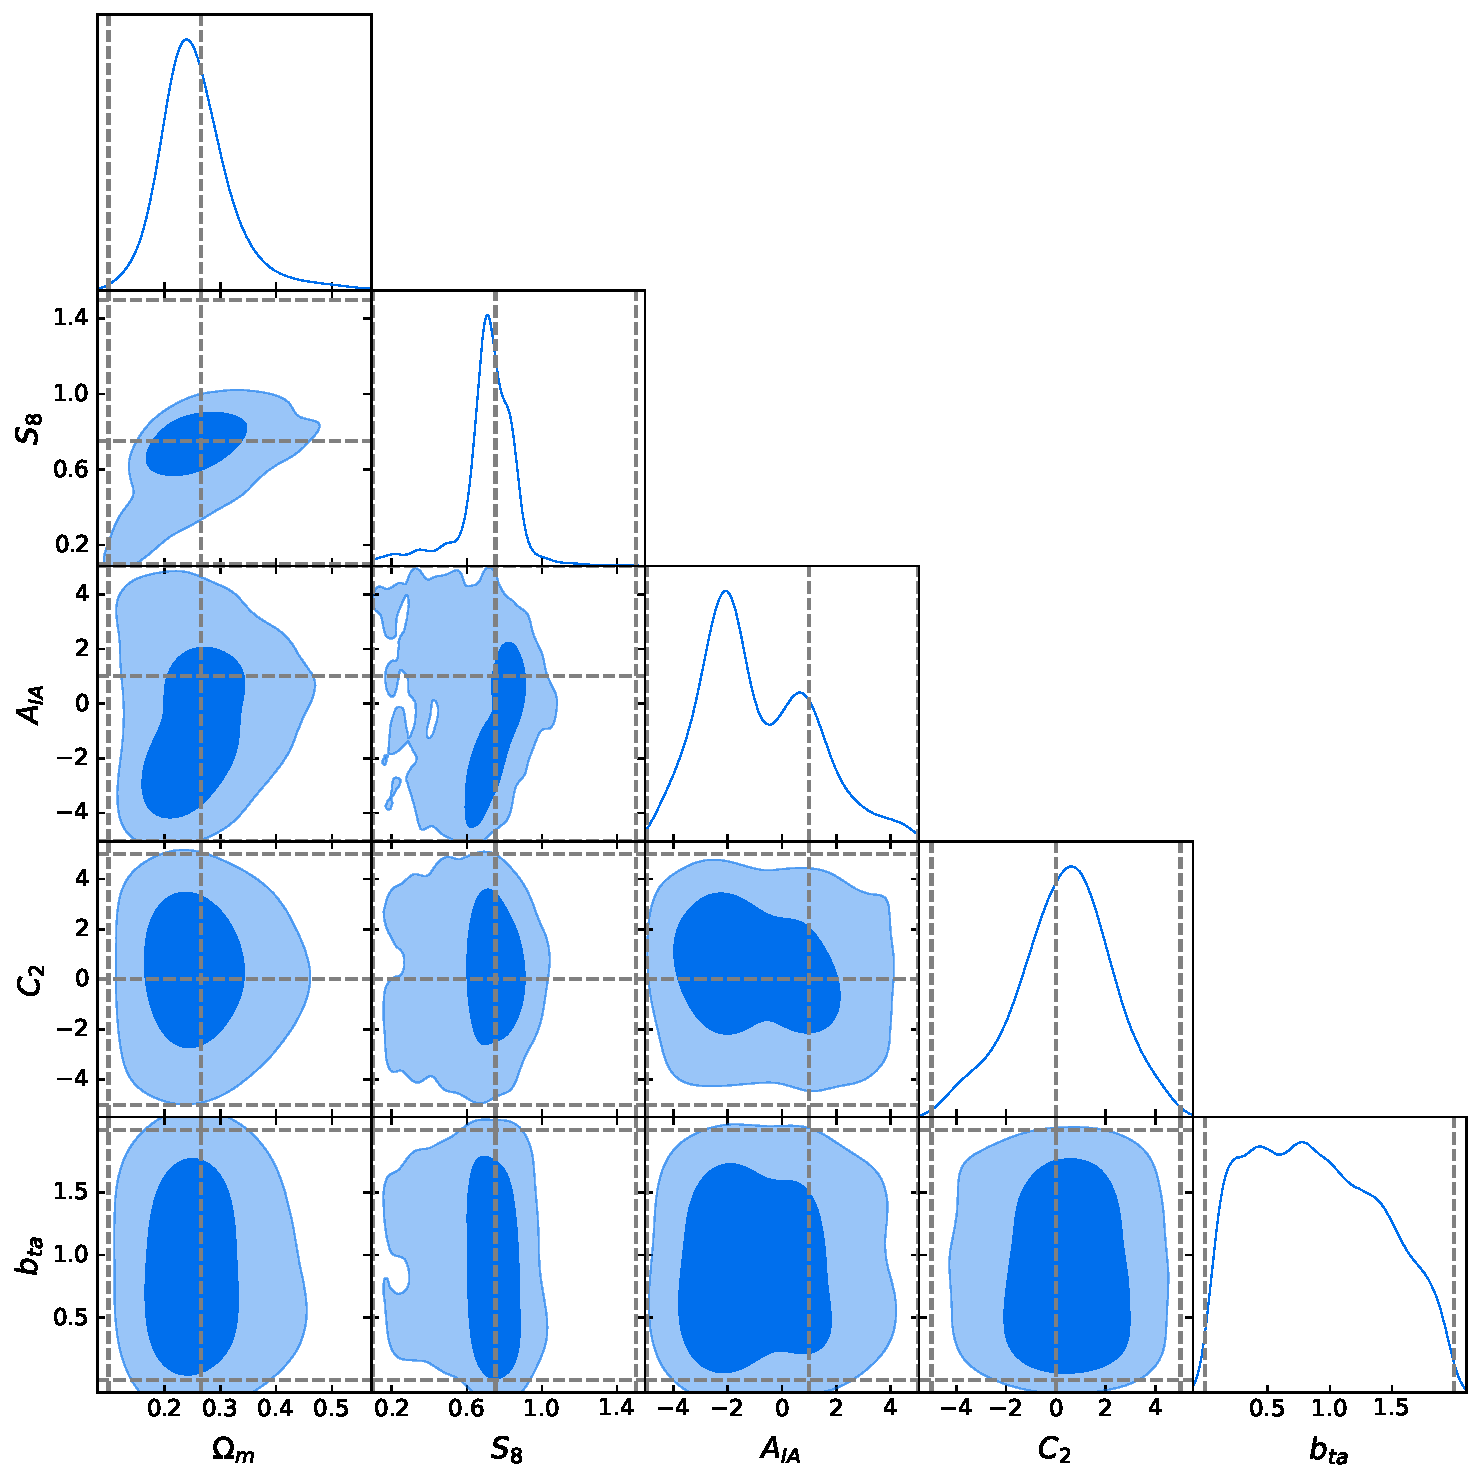
\includegraphics[width=\columnwidth]{graphs/triangle_nla_5D.pdf}
%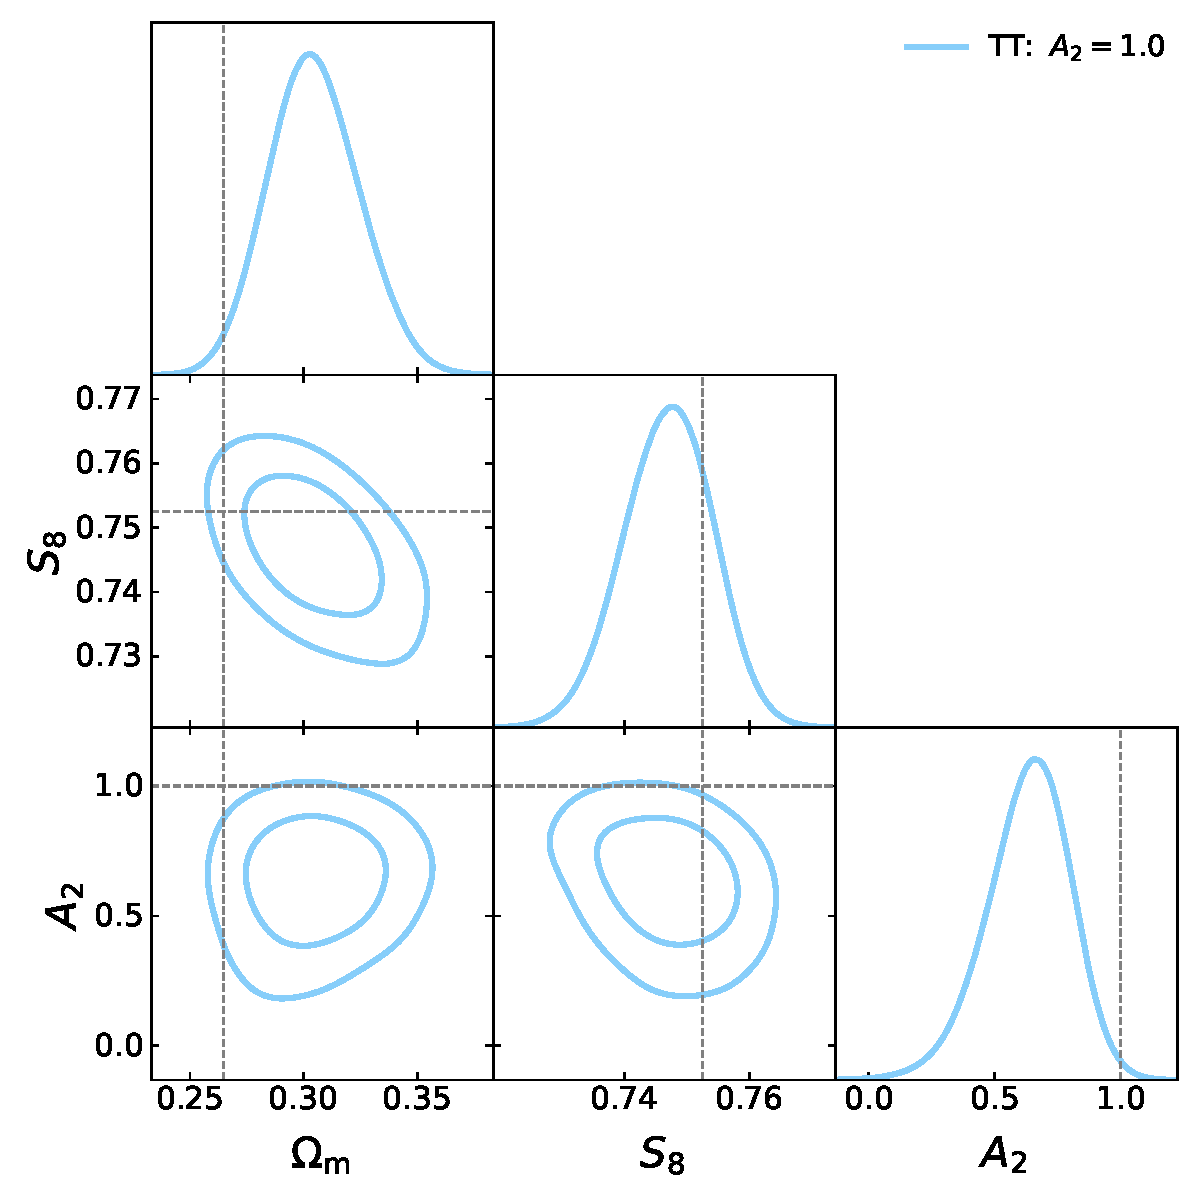
\includegraphics[width=\columnwidth]{graphs/TT_a2.pdf}
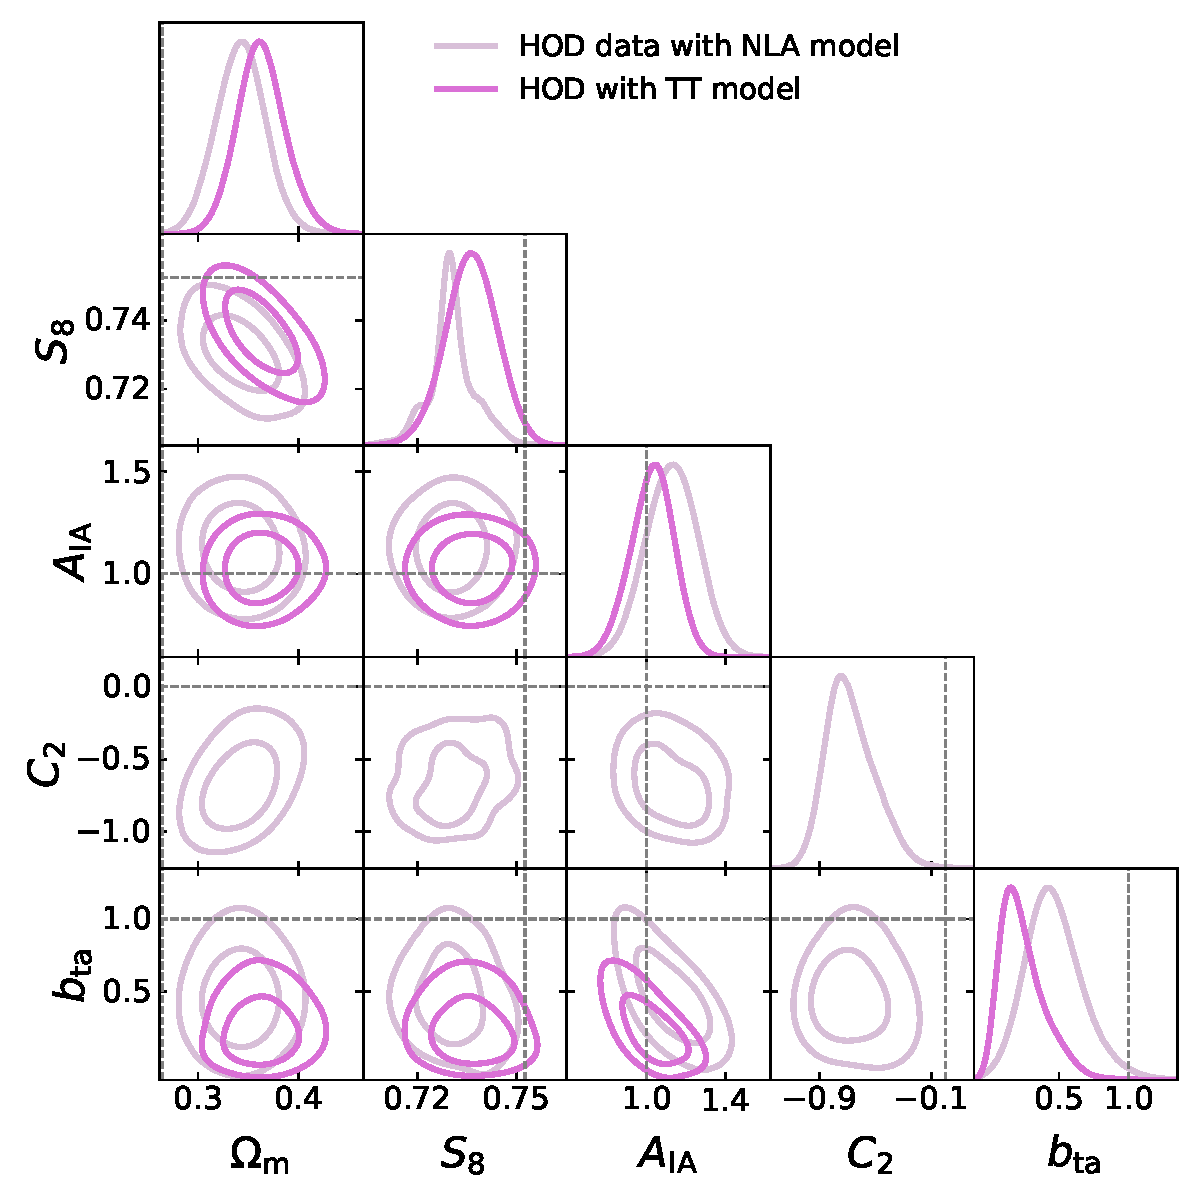
\includegraphics[width=\columnwidth]{graphs/HOD_NLA.pdf}
\caption{Cosmological inference from the HOD-NLA-infused simulations, where either all three TATT parameters are varied (light pink), or keeping $C_2=0$ fixed (dark pink) {\it (Niko, we need to confirm this, adjust the legend...)}.}
\label{fig:triangle_HOD_NLA_combo}
\end{figure}
 \begin{figure}
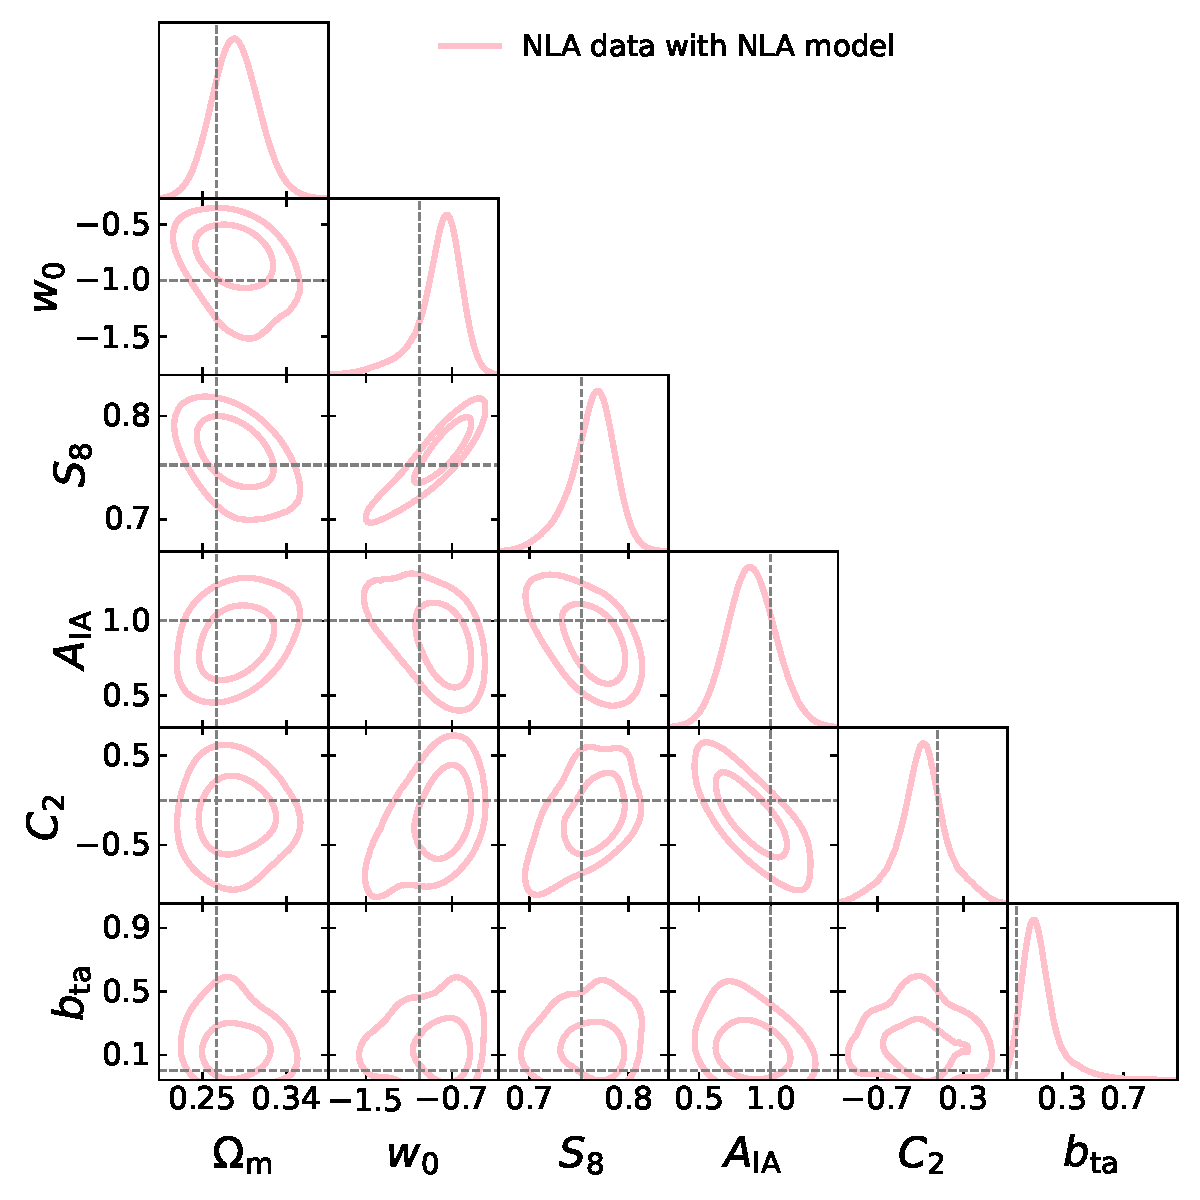
\includegraphics[width=\columnwidth]{graphs/NLA_w0.pdf}
\caption{Cosmological inference from the NLA-infused simulations, where all three TATT parameters are varied.}
\label{fig:corner_nla_w0}
\end{figure}

 
 The last section presented comparisons between measured and modelled signal, reaching generally an excellent agreement but highlighting some small differences. In order to quantify the importance of such differences in a cosmic shear analysis, our evaluation metric must be measurements of biases between the true and the inferred cosmological parameter. We achieve this by running nested likelihood sampling chains with {\sc multinest} \citep{Multinest}, which returns the posterior distributions $\mathcal{P}$ on the cosmological parameters $\boldsymbol \pi$ given a data vector $\boldsymbol  d$, a model vector $\boldsymbol m$, a covariance matrix C, and likelihood function $\mathcal L$ and a set of priors on the inferred parameters.  More precisely, we use a multivariate Gaussian likelihood, and ignore the standard cosmic shear systematic effects caused by photometric redshift errors, shape calibrations or baryon feedback \citep[see][for a recent example]{DESY3-KiDS1000}. We vary a subset of the vanilla $\Lambda$CDM cosmological parameters to establish the general accuracy; increasing the number of varied parameters can lead to a number of projection effects that complicate the interpretation. We therefore focus on varying the parameters best measured by lensing, namely $S_8$, $\Omega_{\rm m}$ and the IA parameters ($A_{\rm IA}, b_{\rm TA}, C_2$). We adopt wide flat priors for all of these, as detailed in Table \ref{table:priors}. 

With the precision of the Rubin data, small fluctuations in the data vectors can lead to significant shifts in the inferred cosmology, which is statistically  expected but makes the IA validation exercise more difficult to interpret. We therefore run our likelihood analyses on  the lowest three redshift bins, deliberately excluding the highest two as they contribute mostly to cosmological information, while we want here to learn more about the recovery of the IA sector. For the same reason we ignore shape noise here, which would only create additional scatter in the posteriors. We additionally exclude angular bins where the models probes highly non-linear scales, and select $\vartheta \in [2 ; 200]$ arcmin for $\xi_+$, and $\vartheta \in [20 ; 400]$ arcmin for $\xi_-$. These scales are highly affected by other systematic effects such as baryonic feedback \citep[see, e.g.][]{Semboloni11, HWVH15, 2020arXiv200715026H} and hence are often removed from the data vectors \citep[as in][]{DESY3_Amon}.

 The projected posteriors  are presented in Figs. \ref{fig:corner_nla_combo}-\ref{fig:corner_deltatt}, analysing simulated data from the six models introduced in Sec. \ref{sec:IA_th} model. In absence of IA contamination the inference from the simulated data is expected to yield posteriors on the cosmological parameters that are consistent with the input truth but not necessarily centred on it due to sample variance. We further dissect the analyses by varying either  one or  all three TATT parameters, highlighting some of the interesting degeneracies.   When analysing the NLA-infused data (Fig. \ref{fig:corner_nla_combo}), all cosmological and IA  parameters are accurately recovered, both for the NLA and TATT modelling. In the later case, the inferred values for $b_{\rm TA}$ and $C_2$ are consistent with zero, but we observe a strong degeneracy between  $A_{\rm IA}$ and  $C_2$ as also found in e.g. \citet[][\it  cite other papers?]{Paopiamsap2024}. 
The inferred  $\Omega_{\rm m}$ is slightly shifted to higher values, however this is not surprising given that cosmic shear alone is generally not able to constrain this parameter. $S_8$, however,  is well recovered, slightly on the high side. As expected, opening up the full TATT parameter space slightly degrades the constrains on cosmology, but no large shifts are observed. The $w$CDM chains also show an excellent convergence, as shown with the pink contours. {\it [update colour, merge figures 11 and 16]}.
 

 We next analyse the TT data with the TATT model in Fig. \ref{fig:triangle_tt_combo}, and  observe an accurate recovery of  $\Omega_{\rm m}$ and $S_8$, however the IA sector is strongly affected by the [$A_{\rm IA}; C_2$] degeneracy, which  pulls the posterior towards the NLA model, with values of $C_2$ consistent with 0 and preferring $A_{\rm IA}\sim 0.5$. When fixing $A_{\rm IA}$ and $b_{\rm TA}$ to the input truth however, the inferred $C_2$ just undershoots the input, pointing to residual differences between our implementation of the TT model and that calculated by TATT. Nevertheless, the fact that the cosmology is well recovered is promising, since ommiting completely the IA modelling would yield to catastrophic biases in $\Omega_{\rm m}$ and $S_8$. 


 As explained above, the extended NLA model infused in our simulations is not entirely well captured by the {\sc CosmoSIS} implementation, especially the $II$ term for the lowest redshift bins. This causes problems when inferring parameters with  {\sc CosmoSIS}, since the predictions attempt to compensate the difference in the IA model, leading to biases in the other parameters. Fig. \ref{fig:triangle_deltaNLA_combo} shows exactly this, failing to infer correctly most parameters. In this particular case,  $\Omega_{\rm m}$ and $S_8$ are only off by $2\sigma$, $A_{\rm IA}$ and $C_2$ are biased by 4-5$\sigma$, however $b_{\rm TA}$ is within 1$\sigma$. The $\delta$-TT model is even more affected by mis-modelling, with a 3$\sigma$ shift in both $\Omega_{\rm m}$ and $S_8$, as seen in Fig. \ref{fig:corner_deltatt}.
 
The infusion with the HOD-NLA model shows much larger deviations, largely driven by the sharp upward turn observed in auto-correlation at low redshifts, which also caused biases on the extended NLA. This causes biases of 2-3$\sigma$ in the cosmological parameters, notably lower $S_8$. In other works, if the  real world IA model was the extended-NLA or HOD-NLA and that we'd analyse it with the {\it cosmoSIS} implementation of  NLA or TATT, this would significantly contribute toward the existing $S_8$ tension \citep{S8tension}, in the same direction currently observed (i.e. late-time probes observe a lower $S_8$ value compared to CMB probes). We are careful here not to claim that this is the single cause of the current tension, but clear mis-model in the IA sector could contribute significantly. We do not include inference of the HOD-TT here since the level of mismatch is even worst.
  
 To summarise this section, aside from the NLA and TT, the infused IA models include terms that are different from the theory and hence lead to significant biases both in the cosmology and IA parameters.  
% We also show in Fig. \ref{fig:corner_nla_w0} the impact of promoting our $\Lambda$CDM inference to a $w$CDM inference, varying the dark energy  equation-of-state parameter $w$ in the range $[-2; -0.3]$. 
 These tests complete our validation of the IA-infusion pipeline, and we now look in the next section at the impact of IA on the weak lensing higher-order statistics mentioned in Sec. \ref{subsec:beyond-2pt}.
 